\documentclass[a4paper,11pt]{article}

\usepackage[ngerman]{babel}

\usepackage{url}
\usepackage{abstract}
\usepackage{graphicx}
\usepackage{booktabs}
\usepackage{float}
\usepackage{tabularx}
\usepackage{amsmath}
\usepackage{hyperref}
\usepackage{listings}
\usepackage{color}
\usepackage{xcolor}
\usepackage{todonotes}
\usepackage[binary-units]{siunitx}
\usepackage{hyphenat}
\usepackage{fontspec}
\usepackage{todonotes}
\usepackage{longtable}
\usepackage{booktabs}
\usepackage{rotating}
%%\usepackage[bottom]{footmisc} breaks referencing of footnotes idk

\usepackage{tgpagella}
\setmainfont{TeX Gyre Pagella}

\usepackage[top=3cm]{geometry}
\usepackage{parskip} %% Absatz anstatt amerikanischer Einrückung

% configure vertical spacing in lists
\usepackage{enumitem}
\setitemize{partopsep=4pt,parsep=2pt}
\setdescription{partopsep=4pt,parsep=6pt}

\makeatletter
\def\namedlabel#1#2{\begingroup
#2%
\def\@currentlabel{#2}%
\phantomsection\label{#1}\endgroup
}
\makeatother

\definecolor{dkgreen}{rgb}{0,0.6,0}
\definecolor{gray}{rgb}{0.5,0.5,0.5}
\definecolor{mauve}{rgb}{0.58,0,0.82}

\lstset{frame=tb,
    language=Java,
    aboveskip=3mm,
    belowskip=3mm,
    showstringspaces=false,
    columns=flexible,
    basicstyle={\small\ttfamily},
    numbers=none,
    numberstyle=\tiny\color{gray},
    keywordstyle=\color{blue},
    commentstyle=\color{dkgreen},
    stringstyle=\color{mauve},
    breaklines=true,
    breakatwhitespace=true,
    tabsize=3
}

\newcommand{\shellcmd}[1]{\texttt{\footnotesize\$ #1}}

\newcommand{\localauthor}[1]{\color{gray} #1 \normalcolor}

\newcommand{\XXitem}[2]{\item[] \textbf{#1} \phantomsection \label{#2}}

\newcommand{\phantomLabel}[1]{\phantomsection\label{#1}}

\newcommand{\doubletitle}[2]{\title{#1 \\ [1ex] \normalsize #2}}
\newcommand{\extauthor}[2]{\author{#1 \\ \normalsize #2}}
\newcommand{\code}[1]{\texttt{#1}}

\begin{document}

    \begin{titlepage}
        \centering

        $~$

        \vspace{0.2cm} %% Hack for vspace to work

        \Huge \textbf{Feinspezifikation}\\
        \normalsize Vorläufige Abgabe\vspace{0.5cm}

        \Huge Team 2
        \Large

        SEP WS 2021/22

        \vspace{2cm}

        
\includegraphics[width=0.8\linewidth]{graphics/LasEs-logo}

        \vspace{2cm}

        Betreuer:

        \textsc{Prof. Dr. Christian Bachmaier}

        \vspace{1cm}

        \begin{table}[H]
            \centering
            \Large
            \begin{tabular}{ll}
                \toprule
                \textbf{Projektphase} & \textbf{Leiter} \\
                \midrule
                Pflichtenheft & Johann Schicho \\
                Entwurf & Stefanie Gürster \\
                Feinspezifikation & Johannes Garstenauer \\
                Implementierung & Thomas Kirz \\
                Validierung & Sebastian Vogt \\
                \bottomrule
            \end{tabular}
        \end{table}

        \vspace{1cm}

        19. November 2021

    \end{titlepage}

    \pagenumbering{gobble}

    %%\maketitle
    \tableofcontents
    %%\listoftodos

    %% ENDE Titelblatt

    \newpage
    \pagenumbering{arabic}

    \section{Einleitung}\label{sec:einleitung}
    \localauthor{Thomas Kirz}

LasEs ist ein \emph{Submission und Review Management System}, also eine Webseite bei der Wissenschaftler:innen Artikel hochladen können, um von Gutachtern \emph{peer reviewed} zu werden.\\
Auf Basis der Gutachten kann ein \emph{Editor} eines Journals oder einer Konferenz den Artikel für die Veröffentlichung akzeptieren.


    \section{Systemarchitektur}\label{sec:systemarchitektur}
    \localauthor{Johannes Garstenauer}

\subsection{Schichten}\label{arch:schichten}
Diese Anwendung folgt einer Schichtenarchitektur.
\begin{itemize}
    \item Die \emph{view}-Schicht enthält die Komponenten zur grafischen Darstellung.
    \item Die \emph{control}-Schicht enthält die Komponenten zur Steuerung der grafischen Darstellung und Reaktion auf
    Nutzereingaben
    \item Die \emph{business}-Schicht enthält die Komponenten, welche die Anwendungslogik umsetzen.
    \item Die \emph{persistence}-Schicht enthält die Komponenten zum Zugriff auf die Datenbasis.
\end{itemize}
Diese Schichten folgen der \emph{\hyperref[arch:mvc]{MVC-Architektur}} wie in \hyperref[arch:pakdia]{Abbildung 1} dargestellt.
\begin{figure}[h]
    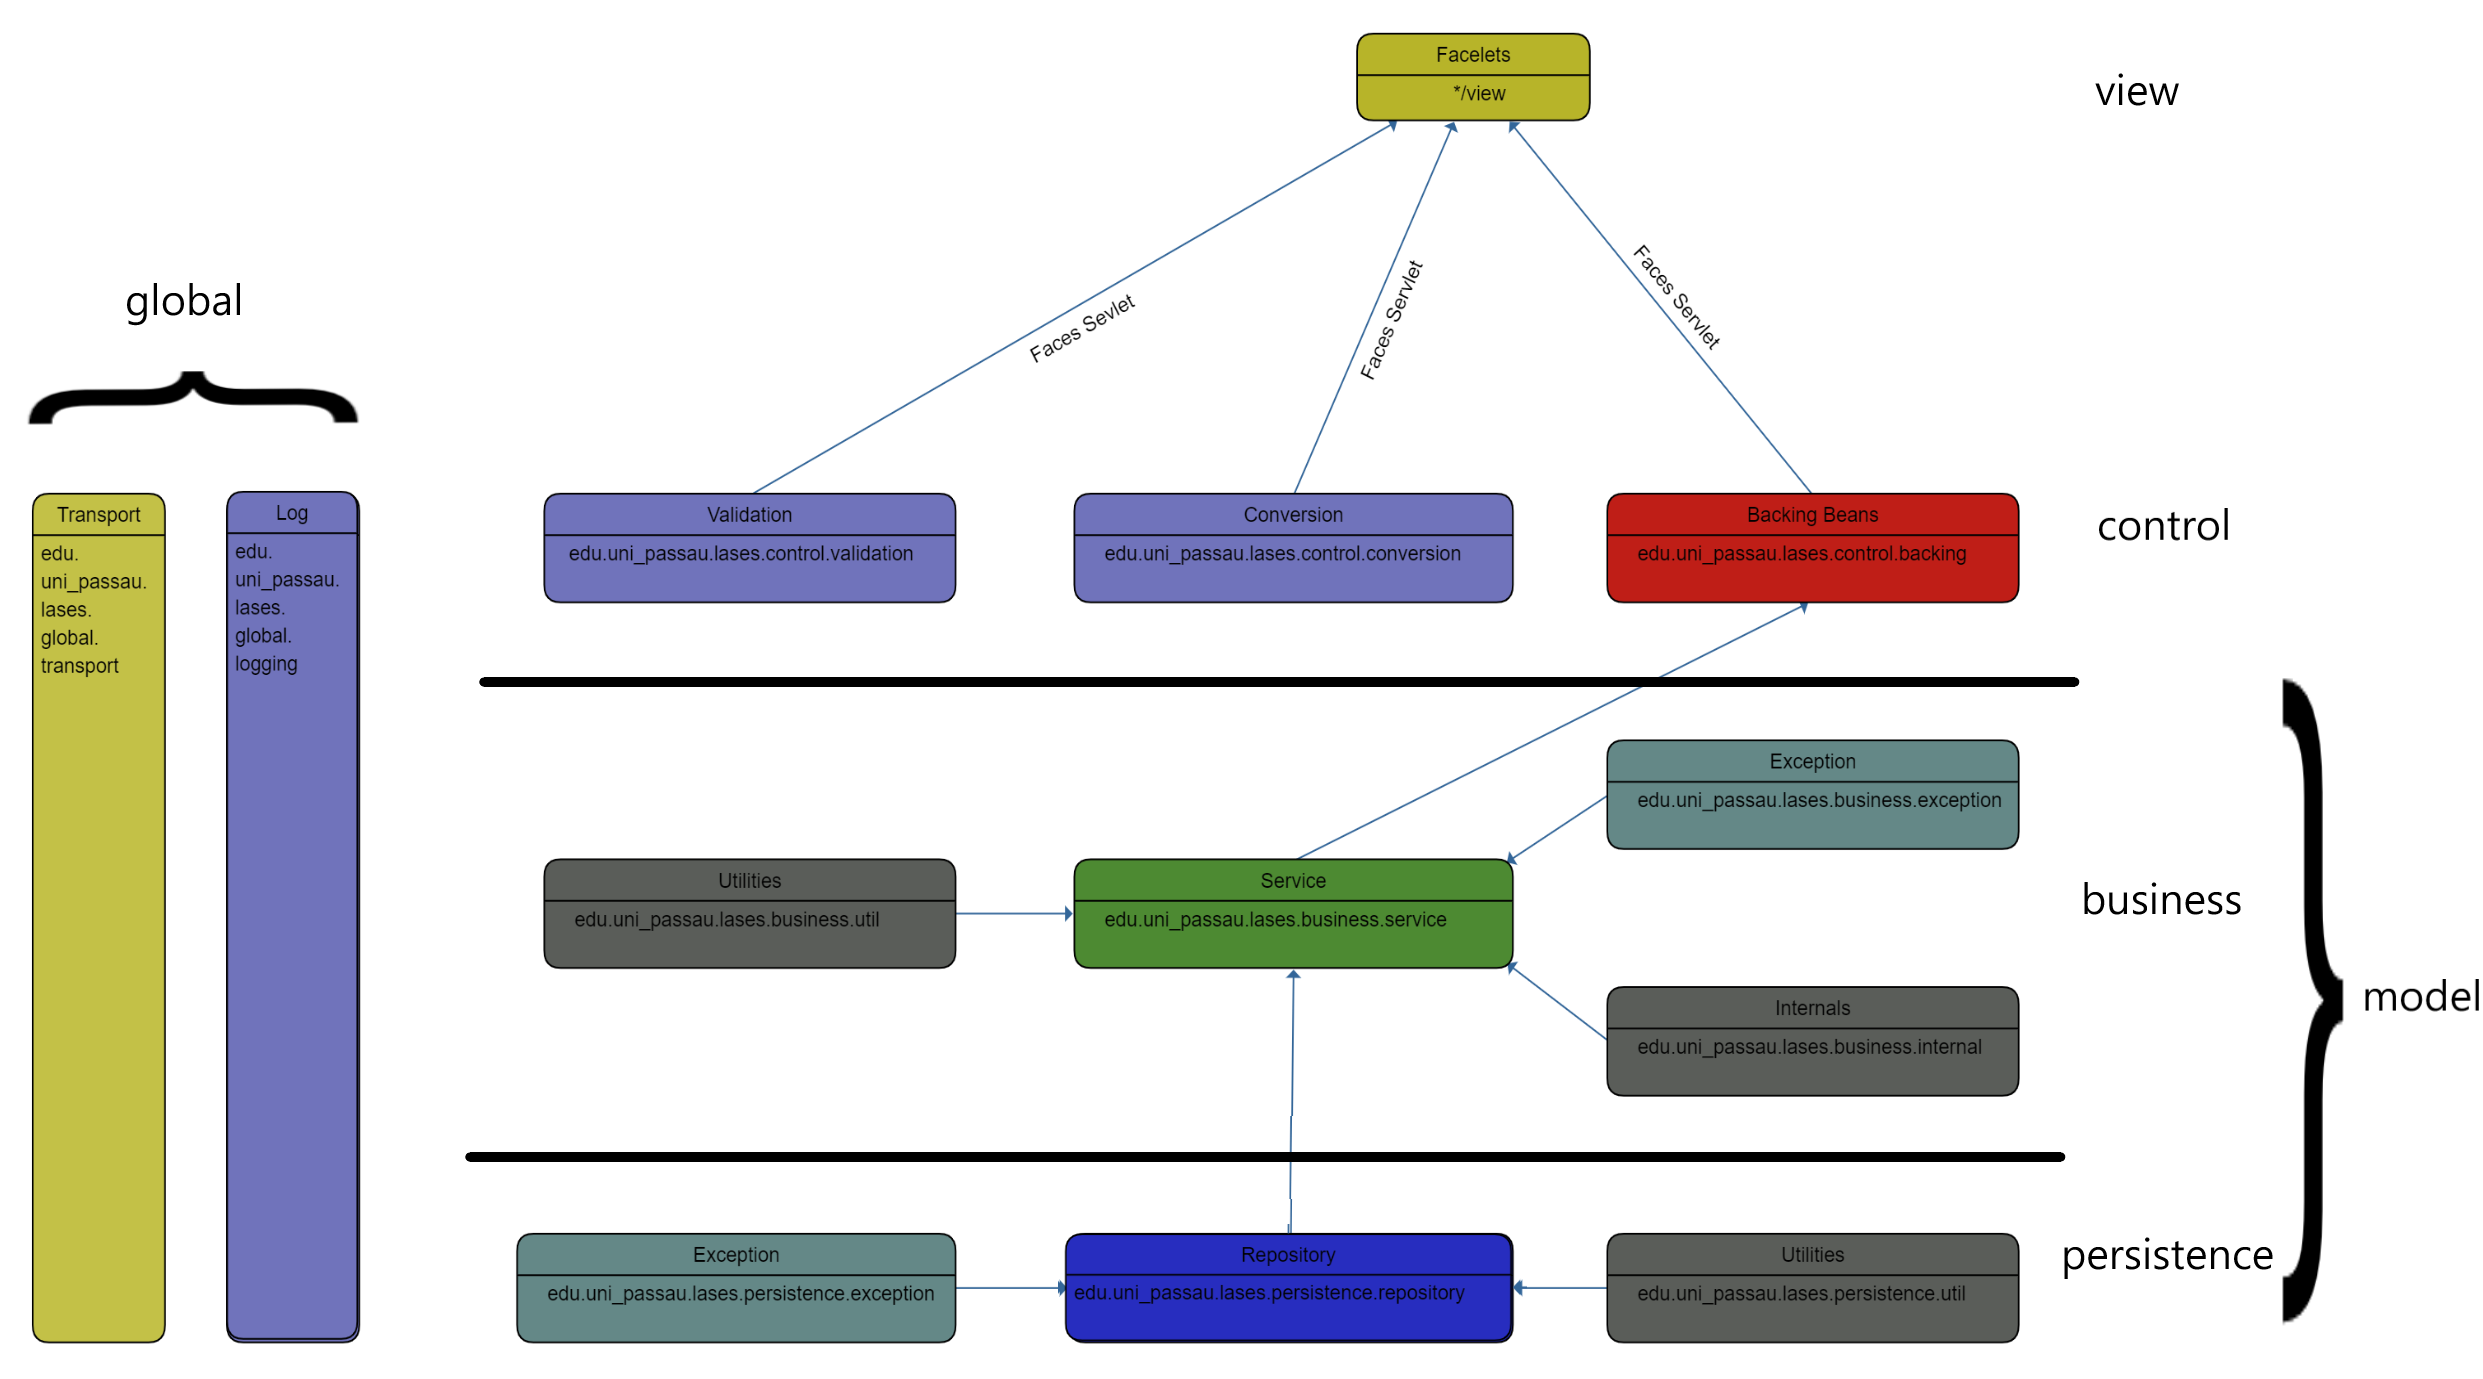
\includegraphics[width=0.85\linewidth]{graphics/Paketdiagramm3.0}\label{arch:pakdia}
    \caption{Das Schichtenmodell der LasEs-Anwendung.}
\end{figure}

%todo mvc sichtbar machen.
%todo view einfügen
%todo servlets?

\subsection{Pakete}\label{arch:pakete}

\subsubsection{edu.uni\_passau.lases.control} \label{arch:control}
Dieses Paket enthält alle Klassen der Kontrollschicht.
\newline\newline
\textbf{\emph{edu.uni\_passau.lases.control.conversion}}
enthält alle Klassen, die zur Konvertierung von Nutzereingaben
in Facelets, verwendet werden.
\newline\newline
\textbf{\emph{edu.uni\_passau.lases.control.validiation}}
enthält alle Klassen die zur Validierung von Nutzereingaben
in Facelets verwendet werden.
\newline\newline
\textbf{\emph{edu.uni\_passau.lases.control.backing}}\label{arch:backing}
enthält alle Managed Beans welche zur Darstellung der Facelets aus der
%todo link
View Verwendung finden. Zu jedem Facelet [facelet] existiert genau ein
Backing-Bean, welches [facelet]Backing genannt wird.
%todo
%\subsubsection*{edu.uni_passau.lases.control.servlet}

\subsubsection{edu.uni\_passau.lases.business}\label{arch:business}
Dieses Paket enthält alle Klassen der Logikschicht.
\newline\newline
\textbf{\emph{edu.uni\_passau.lases.business.service}}\label{arch:service}
enthält alle Klassen, die den Hauptteil der Anwendungslogik umsetzen.
Das sind also alle Dienste welche den
\hyperref[arch:backing]{Backing Beans} zur Verfügung
gestellt werden und auf die auf die %todo link repos
Repositories zugreifen.
\newline\newline
\textbf{\emph{edu.uni\_passau.lases.business.util}}
enthält die Hilfsklassen, welche Dienste zur Verfügung stellen,
die von der Anwendungslogik selbst getrennt werden können.
\newline\newline
\textbf{\emph{edu.uni\_passau.lases.business.exception}} \label{arch:busex}
enthält die Exceptions, die ein Fehlverhalten im System repräsentieren.
\newline\newline
\textbf{\emph{edu.uni\_passau.lases.business.internal}}
enthält die Klassen, welche zur Verwaltung intern verwendet werden.
Hierzugehört beispielsweise die Sessionverwaltung, sowie der Systemstart und -stop.

\subsubsection{edu.uni\_passau.lasses.persistence}\label{arch:persistence}
Dieses Paket enthält alle Schichten der Persistenzschicht.
\newline\newline
\textbf{\emph{edu.uni\_passau.lases.persistence.repository}}\label{arch:repository}
enthält alle Klassen, die dem direkten Zugriff auf die Datenbasis dienen.
\newline\newline
\textbf{\emph{edu.uni\_passau.lases.persistence.util}}
enthält die Hilfsklassen zur Datenbankverwaltung, wie einen
Connection-Pool oder Mailservice.
\newline\newline
\textbf{\emph{edu.uni\_passau.lases.persistence.exception}}
enthält die Exceptions, welche ein Fehlverhalten im Umgang mit der
Datenbasis repräsentieren.

\subsubsection{edu.uni\_passau.lases.global}
Dieses Paket enthält alle Klassen welche über Schichten hinweg
verwendet werden.
\newline\newline
\textbf{\emph{edu.uni\_passau.lases.global.logging}}
enthält Hilfsklassen für schichtenübergreifende Aufgaben, wie das Logging.
\newline\newline
\textbf{\emph{edu.uni\_passau.lases.global.transport}}\label{arch:transport}
enthält alle POJO-Klassen, die Daten in der Anwendung repräsentieren und zu deren
Transport verwendet werden.

%todo i18n resource bundles: info (tooltips), names (labels), messages (facesmsg)

\subsection{Fehlerbehandlung}
Bei Verwendung der Anwendung können Fehler auftreten. Diese werden zur Nachvollziehbarkeit
immer geloggt. Daraufhin wird auf verschiedene Weisen verfahren.

\subsubsection{Geprüfte Ausnahmen}
Geprüfte Ausnahmen repräsentieren Ausnahmesituationen, mit
denen gerechnet werden muss und auf die reagiert werden sollte.
Treten solche auf, dann werden sie mit einer semantisch aussagekräftigen
\hyperref[arch:busex]{Ausnahmeklasse} und Nachricht
an den Aufrufer weiterpropagiert.
In \hyperref[arch:service]{Service-Klassen} werden auftretende Ausnahmen weiter zu den
\hyperref[arch:backing]{Backing-Beans} propagiert, wo FacesMessages %todo link
generiert werden.
Diese werden dann von den zugehörigen Facelets %todo link
gerendert.

\subsubsection{Ungeprüfte Ausnahmen}
Bei ungeprüften Ausnahmen handelt es sich um fatale Fehler, wie sie beispielsweise durch
Programmierfehler entstehen können. Diesen werden vom anwendungsweiten
ExceptionHandler %todo link
aufgegriffen. Der User wird daraufhin auf die Fehlerseite %todo link
weitergeleitet.
Falls in der \emph{web.xml} die \emph{PROJECTPHASE}-Konstante auf \emph{DEVELOP} gesetzt ist,
dann wird der gesamte Stacktrace auf der Fehlerseite angezeigt.
%todo stacktrace wirklich drinnen lassen oder offensichtliche Kopie?

\subsection{Frameworks}\label{arch:frameworks}

\subsubsection{Jakarta Server Faces}
Jakarta Server Faces (JSF; früher JavaServer Faces) ist ein Framework-Standard zur
Entwicklung von grafischen Benutzeroberflächen für Webanwendungen, basierend auf Servlets und JSP-Technik.
Es wird die Referenzimplementierung \emph{Mojarra} verwendet.

\subsubsection{Context and Dependency Injection}
Die \emph{Context and Dependency Injection} ist eine Technologie welche die
Abhängigkeitsverwaltung zwischen Objekten vereinfacht. Im Sinne der
\emph{Inversion of Control} werden dem Entwickler Werkzeuge an die Hand gelegt, mithilfe derer
er Objektrefernzierung tätigen kann, ohne diese Objekte vorher explizit zu erstellen.
Diese referenzierten Objekte können in andere Objekte zur Laufzeit \emph{injiziert} werden.
Somit können Objekte in dieser Anwendung ohne Initialisierung oder umständlichen Transport der Referenzierung
verwendet werden.
Dies ermöglicht eine loosere Kupplung zwischen Klassen und somit Erweiterbarkeit
und Austauschbarkeit.
Das \emph{CDI} verwaltet in dieser Anwendung alle Objekte der \hyperref[arch:backing]{Backing-Beans}
und \hyperref[arch:service]{Services}.
Es wird die Referenzimplementierung \emph{Weld} von \emph{JBoss} verwendet.

\subsection{Patterns}\label{arch:patterns}
%todo konkret auf unser System abstimmen. (Keine allg. erklärung der patterns)

\subsubsection{Model View Controller}\label{arch:mvc}
Dieses Entwurfsmuster trennt die Klassen und Komponenten der Anwendung in drei
verschieden Teile, welche jeweils eigene Aufgaben übernehmen:
\begin{itemize}
    \item Die \emph{\textbf{View-Komponenten}} übernehmen alle Aufgaben,
    welche mit der grafischen Darstellung der Anwendung zusammenhängen.
    In dieser Anwendung sind dies die Facelets. %todo link facelets
    \item Die \emph{\textbf{Controller-Klassen}} übernehmen alle Aufgaben,
    welche die Interaktion zwischen der View und dem Model betrifft. Sie behandeln
    Nutzereingaben, Validation und Konvertierung etc. In dieser Anwendung befinden sie
    sich in den \hyperref[arch:control]{edu.uni\_passau.lases.control} Paketen.
    \item Die \emph{\textbf{Model-Komponenten}} beinhalten die Modelldaten, sowie jene
    Klassen welche sich mit deren Beschaffung und Verarbeitung beschäftigen. In dieser
    Anwendung befinden sie sich in den \hyperref[arch:business]{edu.uni\_passau.lases.business}
    und \hyperref[arch:persistence]{edu.uni\_passau.lases.persistence} Paketen.
\end{itemize}
Die Verwendung dieses Patterns bietet viele Vorteile hinsichtlich der Modularität
und Erweiterbarkeit der Anwendung.

\subsubsection{Singleton}
Eine Klasse, welche nach dem Singleton-Entwurfsmuster implementiert wurde zeichnet
sich dadurch aus, dass es nur genau eine Instanziierung von dieser Klasse geben
kann und darf. Hierdurch werden vorrangig Ressourcen gespart, außerdem wird die
Verwaltung der im Objekt gekapselten Funktionalität erleichtert.
Ein Beispiel hierfür ist der Connection Pool, %todo link und mehr? Config reader
welcher ein Singleton ist damit, unter anderem, sichergestellt wird, dass
eine genau festgelegte Anzahl an Datenbankverbindungen existiert und nicht mehr.

\subsubsection{Data Transfer Object}
Dieses Entwurfsmuster schreibt die Verwendung von \emph{Data Transfer Objects}
zur einheitlichen Darstellung der Entitäten in den Modelldaten und dem Transport
von Daten vor.
Diese sind POJOs, welche private Felder zur Repräsentation der Daten mit Getter- und
Settermethoden haben.
Der Vorteil der Verwendung dieses Entwurfsmusters liegt darin, dass eine
einheitliche und übersichtliche Schnittstelle für Datenrepräsentation und Transport
in der Anwendung besteht. Die zugehörigen Klassen lagern im
\hyperref[arch:transport]{edu.uni\_passau.lases.transport} Paket.

\subsubsection{Repository}
Beim \emph{Repository} Pattern wird für jedes Business-Objekt oder jede Entität
eine Klasse definiert welche den Datenbankzugriff auf die zugehörigen Daten steuert.
Für diesen Zugriff werden oft die \textit{CRUD}-Methoden, das heißt
\begin{itemize}
    \item \textit{CREATE} zur Erstellung,
    \item \textit{READ} zum Erhalten,
    \item \textit{UPDATE} zum Updaten,
    \item und \textit{DELETE} zum Löschen
\end{itemize}
eines oder mehrerer Datenbankeinträge der zugehörigen Entität, angeboten.
Weiterhin findet das Mapping auf die \hyperref[arch:transport]{DTO-Objekte} dieser Anwendung statt.
In dieser Anwendung finden sich die \emph{Repository-Pattern} Klassen im Paket
\hyperref[arch:repository]{edu.uni\_passau.lases.repository}. Durch die mit
der Verwendung dieses Patterns gewonnenen Übersichtlichkeit erleichtern wir uns die
Implementation und ermöglichen leichte Erweiterbarkeit der Datenschemas.

\subsubsection{Object Pool}
Das \emph{Object Pool} Erzeugungsmuster wird dazu verwendet, Objekte nach initialer Erzeugung
vorzubehalten, da sinnvoller ist als sie bei jeder Verwendung neu zu erzeugen.
Somit werden Ressourcen gespart. In dieser Anwenfung findet dieses Entwurfsmuster
beim Connection Pool %todo link
Verwendung und bietet den zusätzlichen Vorteil, dass eine feste Maximalanzahl an
Datenbankverbindungen festgelegt werden kann.

\subsubsection{Observer}
Das \emph{Observer} Verhaltensmuster beschreibt Methoden, welche auf
Änderungen im Zustand eines Systems warten und daraufhin handeln.
In unserem System findet das beispielsweise beim LifeCycleListener %todo link
zur Reaktion auf das Herunterfahren oder Starten des Systems Verwendung.
%todo propagation der messages aus service in backingbeans

    \section{Klassendiagramm}\label{sec:klassendiagramm}
    \localauthor{
	\begin{itemize}
		\item RSA: Sebastian Vogt
		\item Control Schicht: Sebastian Vogt
		\item Business Schicht: Johannes Garstenauer
		\item Persistence Schicht: Sebastian Vogt
		\item Cross-Cutting Concerns: Sebastian Vogt
	\end{itemize}
}

\newcommand{\classtable}[1]{\begin{longtable}[H]{m{5cm}m{9cm}}
                                \hline
                                \textbf{Klassenname} & \textbf{Beschreibung} \\
                                \hline
                                \hline
                                #1
\end{longtable}
}

\newcommand{\classentry}[2]{\textbf{#1} & #2 \\
	\hline
}

\subsection{Klassendiagramm}

Im folgenden Klassendiagramm wurden folgende Konventionen verwendet:
\begin{itemize}
    \item Properties sind als private Attribute modelliert.
    Konstruktoren sind ausgespart.
    \item Referenzattribute auf andere Klassen des Diagramms sind als Pfeile dargestellt.
    Diese haben standardmäßig keine Getter und Setter, außer anders angegeben.
    \item Konstruktoren sind ausgespart, außer dieser ist privat.
    \item In den Backingbeans sind Attribute, die lediglich einen Anzeigetext aus einem Ressourcebundle laden, nicht angegeben.
    \item Gestrichelte Pfeile sind \emph{use-Pfeile}, egal ob diese mit \emph{<<use>>} versehen sind oder nicht.
\end{itemize}

Weitere Informationen zur Interpretation des Diagramms finden sich in den jeweiligen Packages.

\begin{figure}[H]
	\centering
	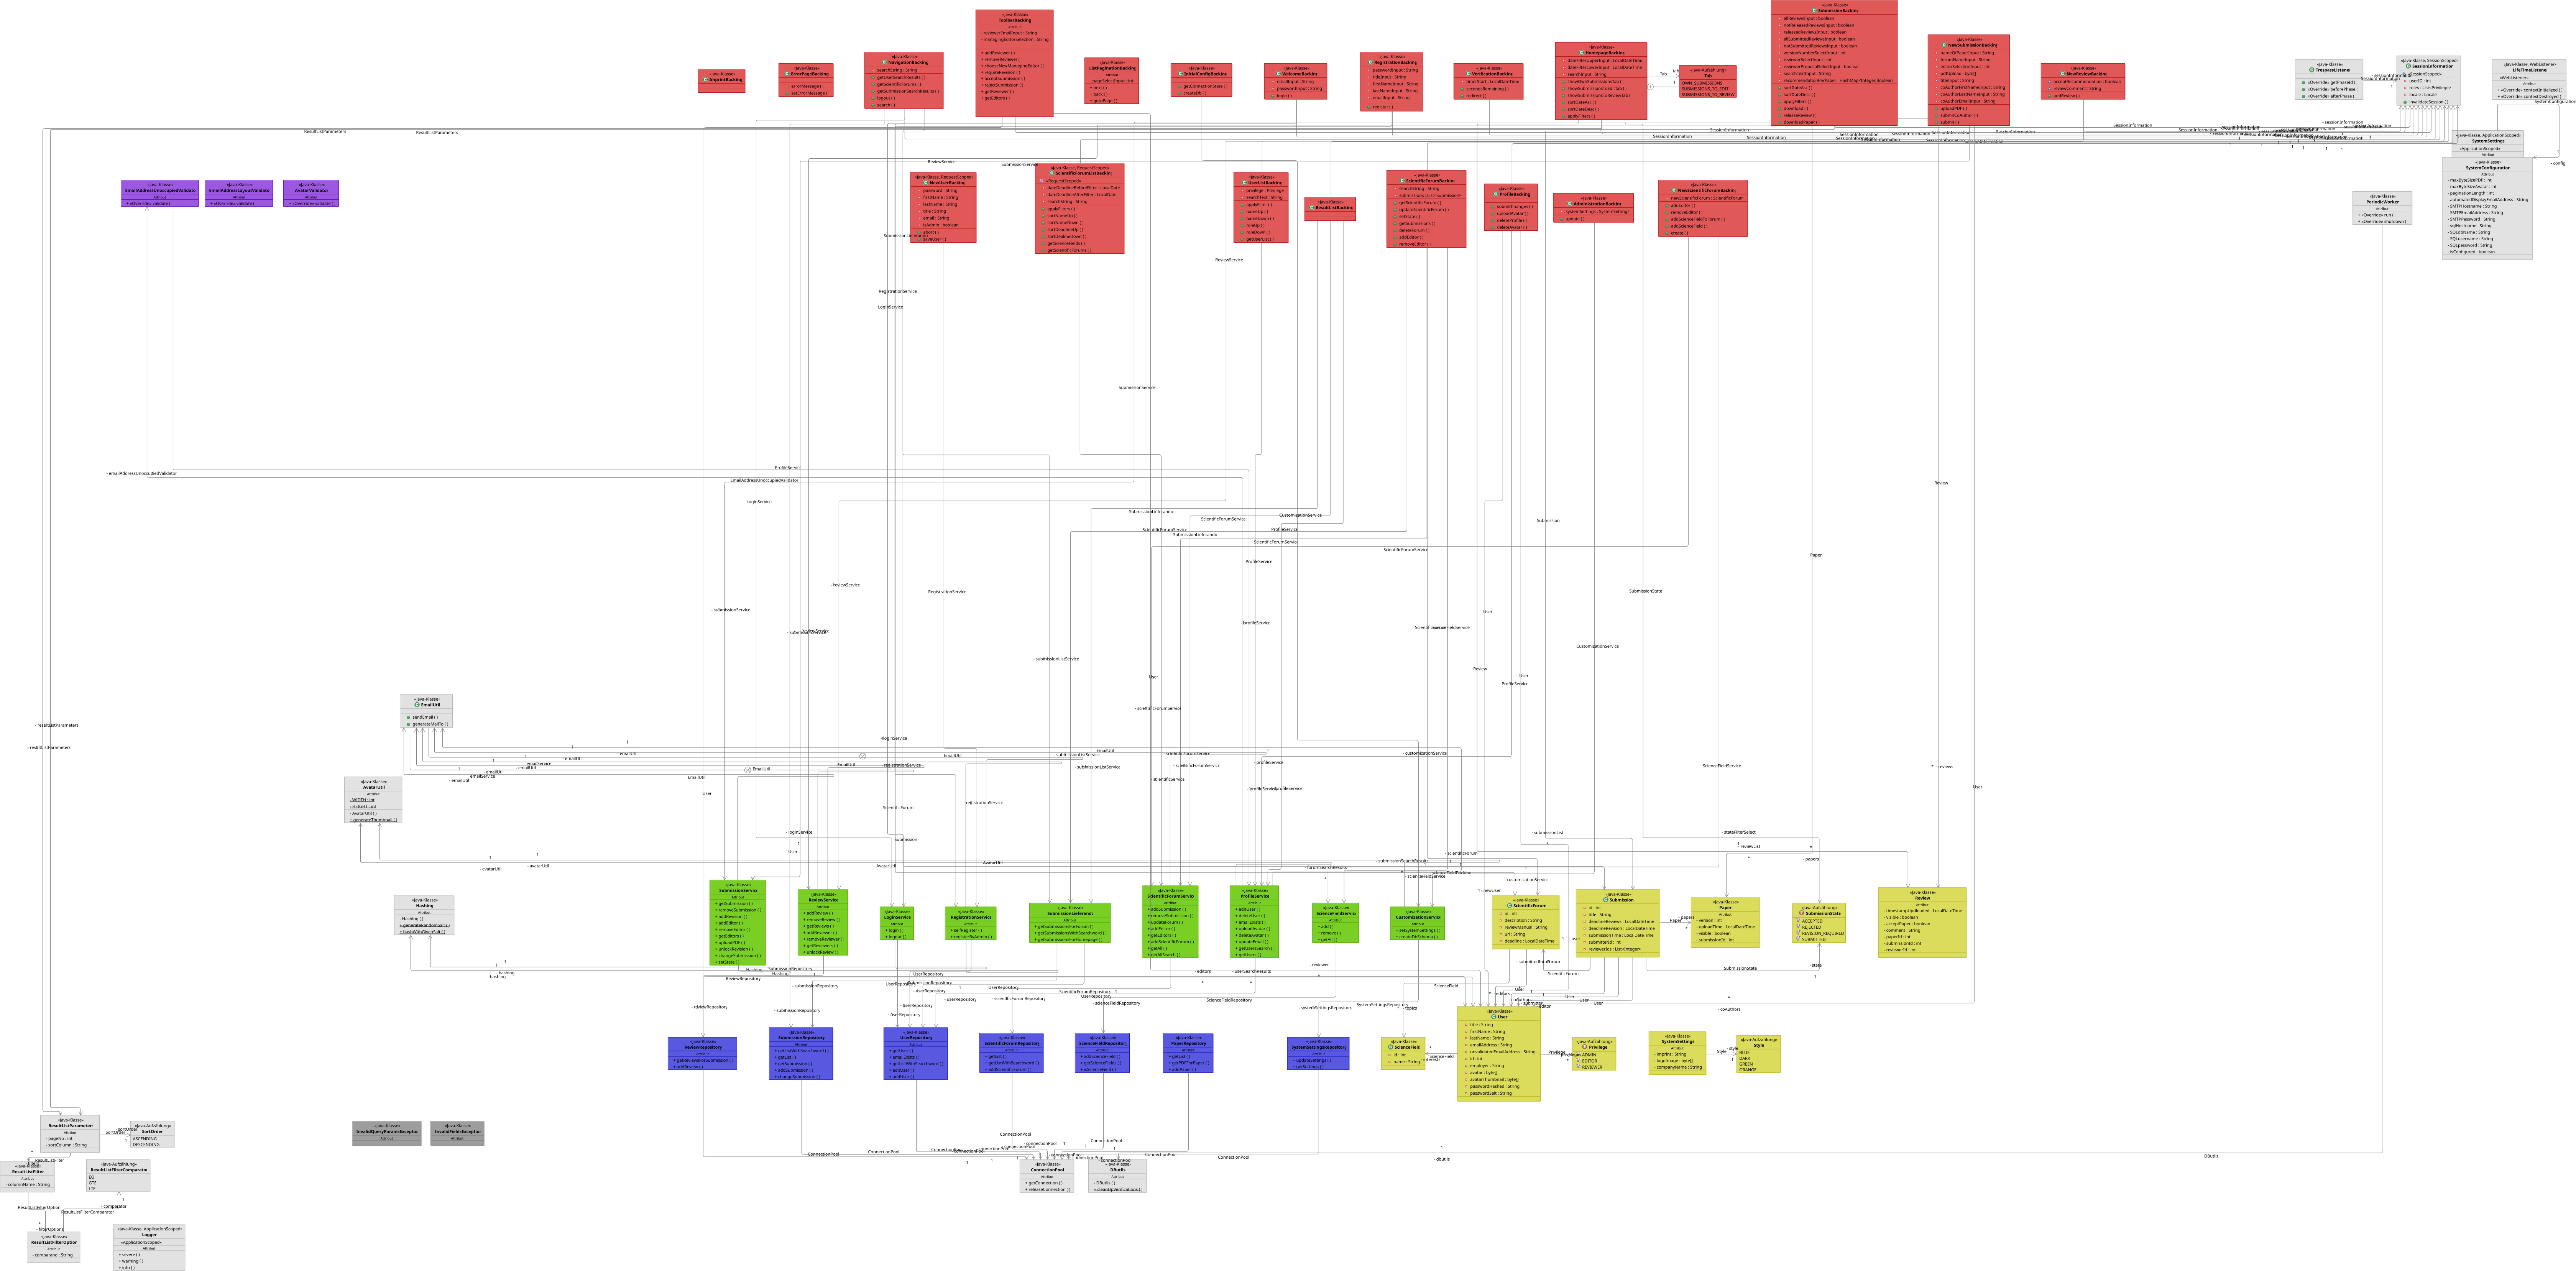
\includegraphics[width=\linewidth]{graphics/klassendiagramm_png}
\end{figure}

% Hier Klassendiagramm mal irgendwann einfügen.

\subsection{Klassenbeschreibungen}

\subsubsection{de.lases.global.logging}

\begin{figure}[H]
	\centering
	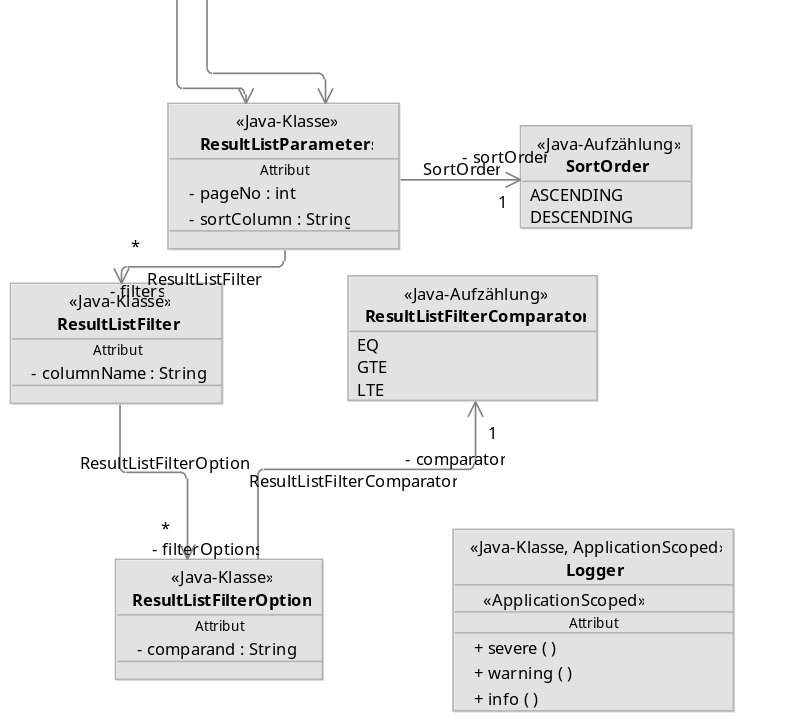
\includegraphics[height=3cm]{graphics/global_util}
\end{figure}

\classtable{
	\classentry{Logging}{This Logger allows logging in different log-levels.}
}

\subsubsection{de.lases.global.transport}

Im folgenden Diagramm gilt für die Klassen mit dickem schwarzem Rand folgende Konvention:
\begin{itemize}
	\item Die Zuordnungen zwischen den Klassen werden nicht durch Java Zeiger realisiert, sondern durch Speichern der Id des jeweiligen Objekts.
	\item Bei einer $x \rightarrow 1$ Beziehung (mit $x \in \{1, *\}$) merkt sich das Objekt auf der Linken Seite die Id des zugeordneten Objektes
	\item Bei einer $x \rightarrow *$ Beziehung merkt sich das Objekt auf der Linken Seite \emph{keine} Liste der zugehörigen Ids. Zuordnungen sind in diese Richtung also nicht unmittelbar traversierbar.
\end{itemize}

\begin{figure}[H]
	\centering
	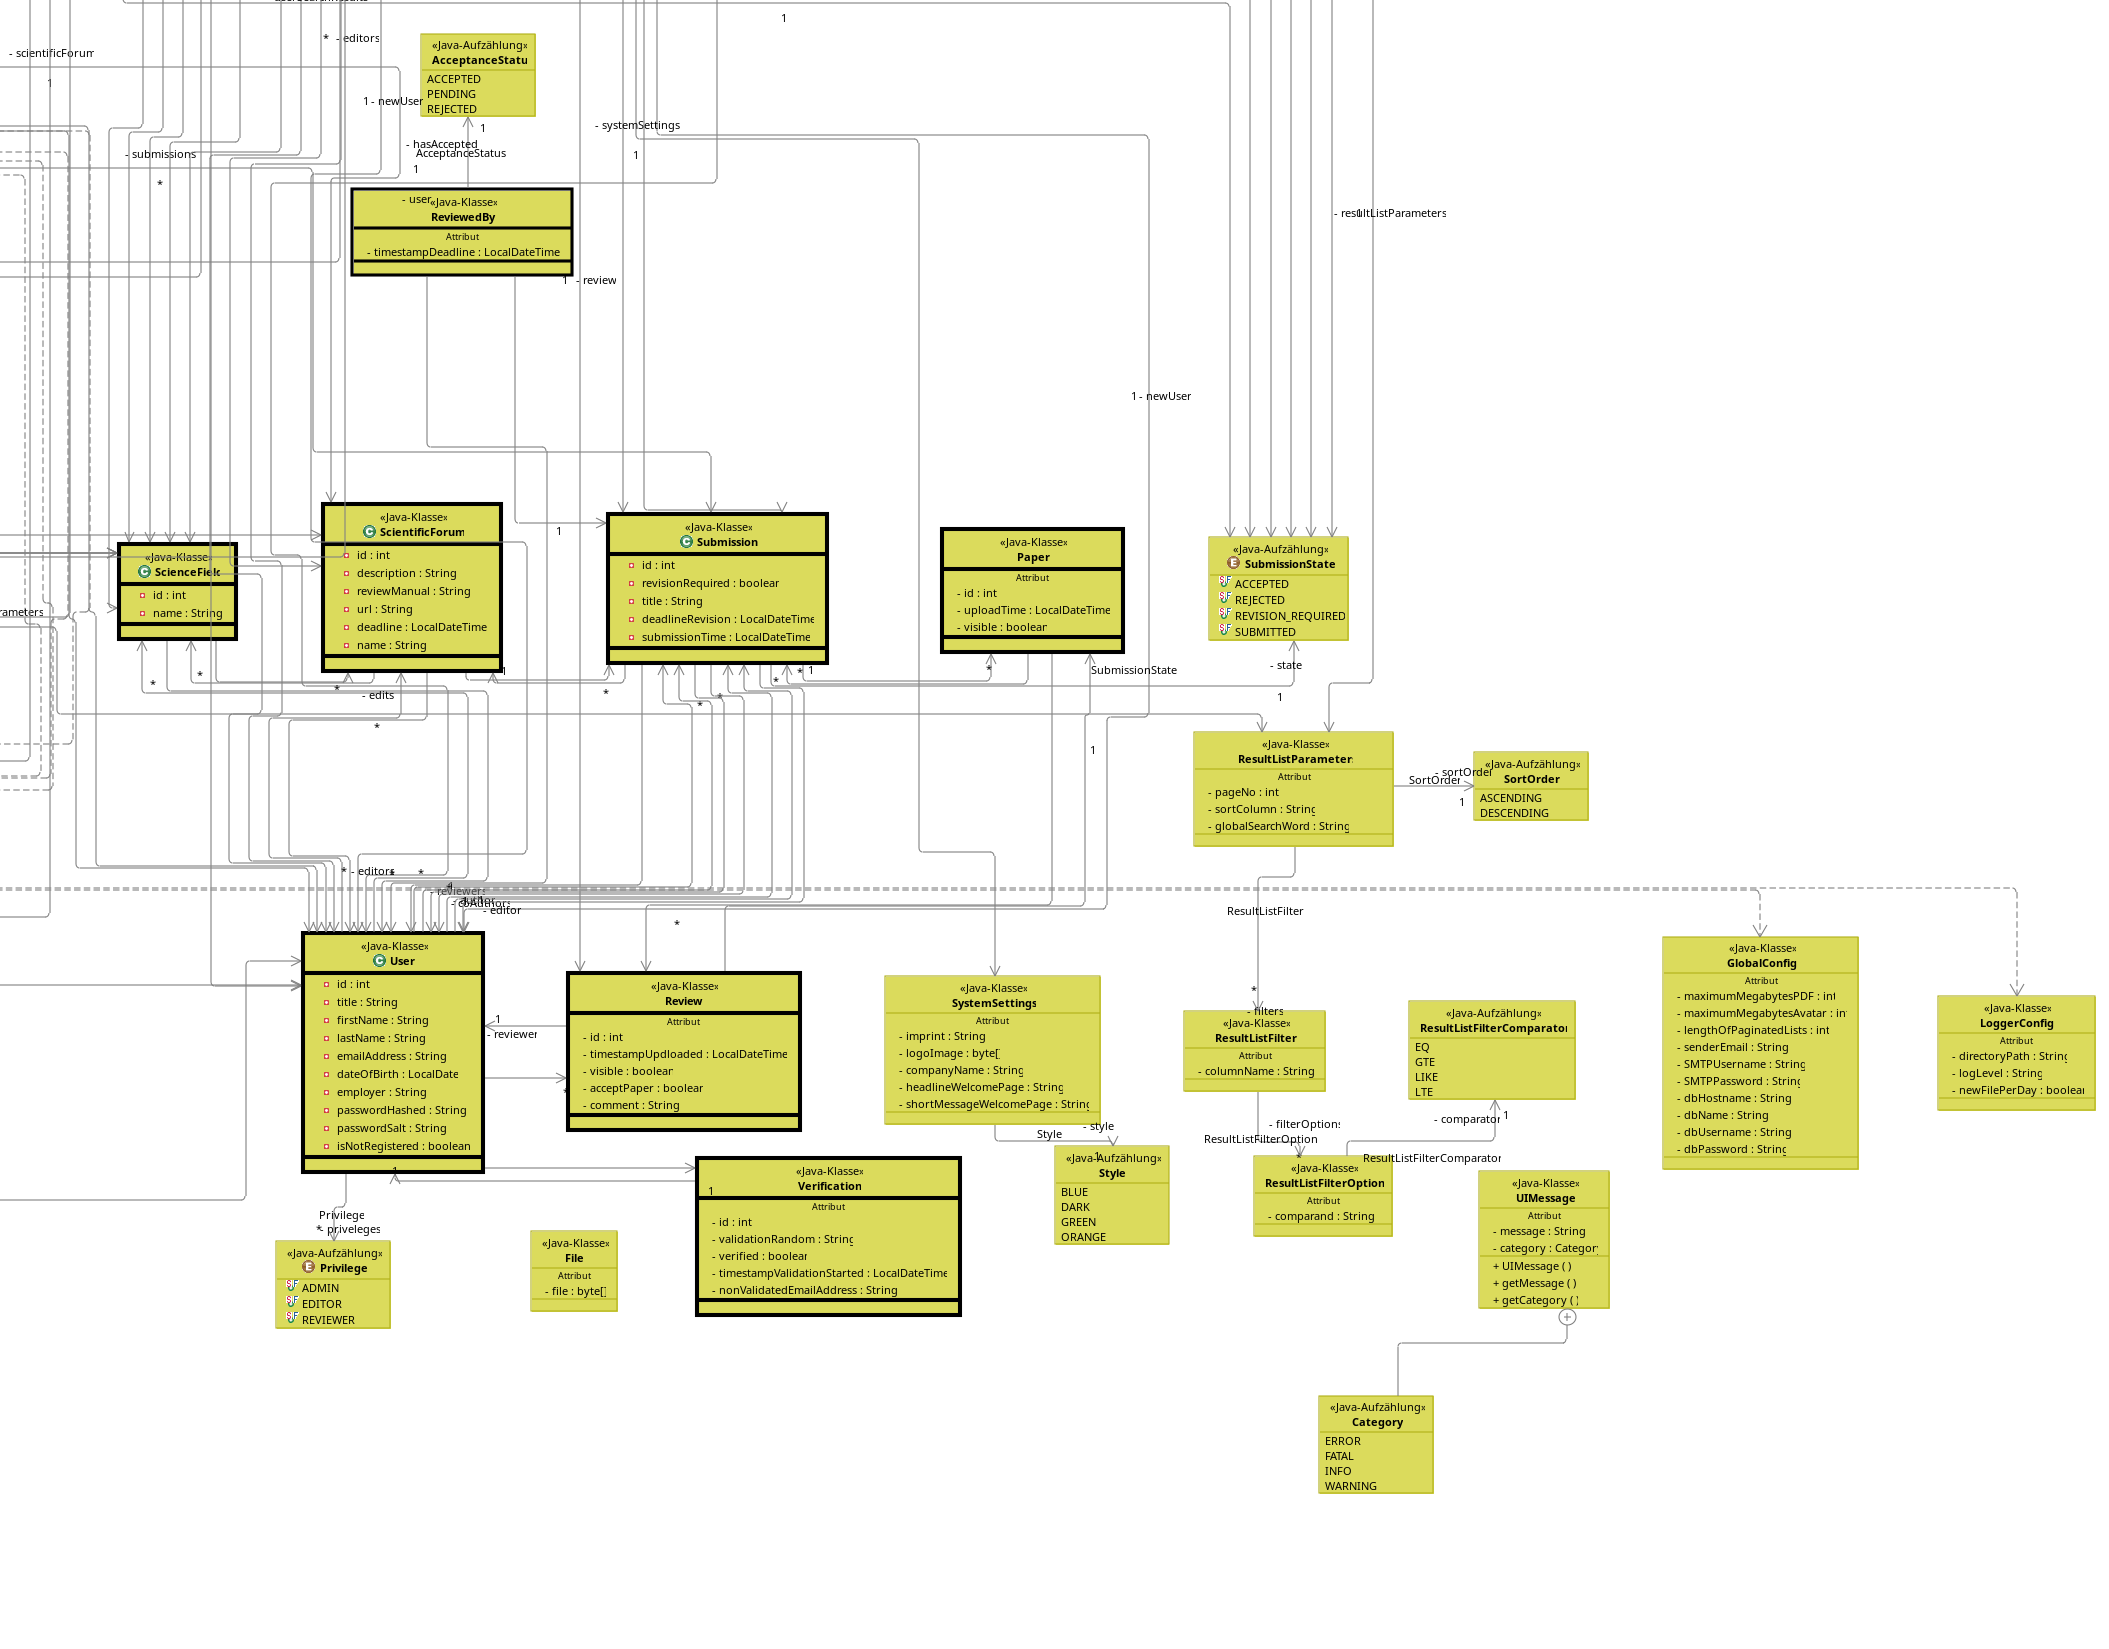
\includegraphics[height=3cm]{graphics/global_transport}
\end{figure}

\classtable{
	\classentry{Paper}{This DTO represents a paper.}
	\classentry{Privilege}{This represents a user privilege.}
	\classentry{Review}{This DTO represents a review.}
	\classentry{ScienceField}{This DTO represents a field of Science.}
	\classentry{ScientificForum}{This DTO represents a forum}
	\classentry{Style}{This represents a user interface style.}
	\classentry{Submission}{This DTO represents a submission.}
	\classentry{SubmissionState}{This represents a submissions state.}
	\classentry{SystemSettings}{This DTO represents the system settings.}
	\classentry{User}{This DTO represents a user.}
	\classentry{ResultListParameters}{This class bundles parameters for requesting lists from the database. This includes page numner, sorting of the results and filtering of the results}
	\classentry{SortOrder}{A List can be sorted in ascending or descending order}
	\classentry{ResultListFilter}{A filter that can be applied on a column of a table}
	\classentry{ResultListFilterOption}{A single comparison that can be used to construct a ResultListFilter}
	\classentry{ResultListFilterComparator}{The three comparators equal to, less than or equal and greater than or equal}
	\classentry{GlobalConfig}{Holds all data that is read from the config file.}
	\classentry{Verification}{Bundles information about the verification process is somebody is newly registered or has just changed theirq email.}
	\classentry{File}{Encapsulates a file that is passed between the layers.}
}

\subsubsection{de.lases.control.backing}

\begin{figure}[H]
	\centering
	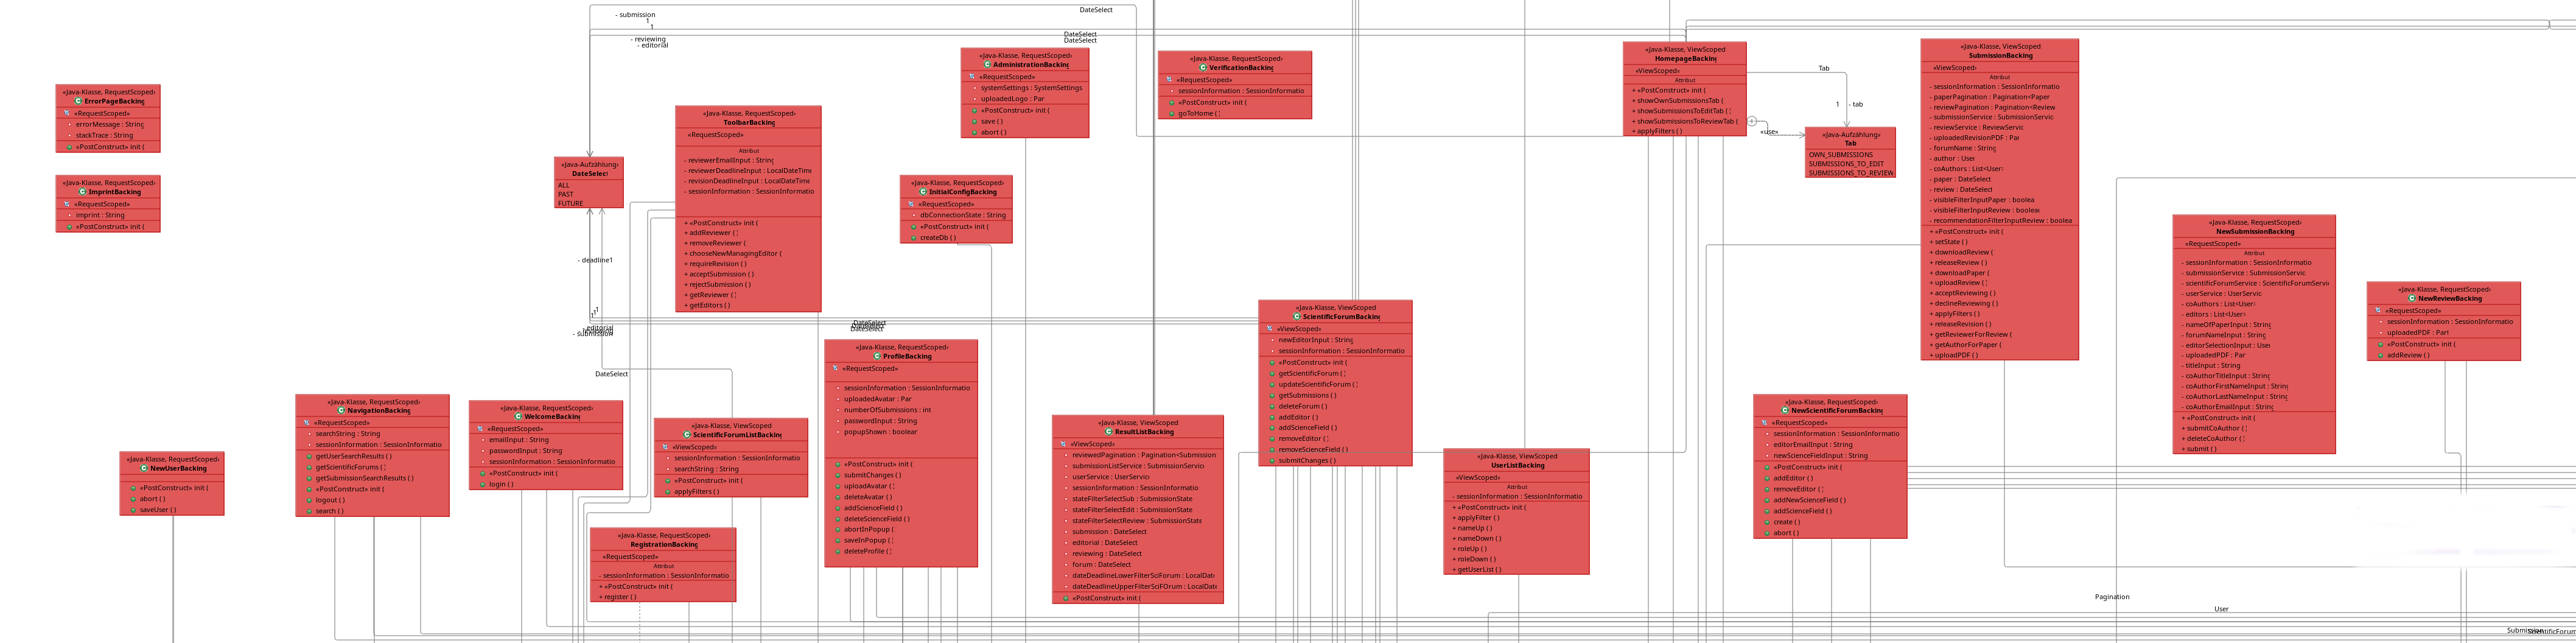
\includegraphics[width=0.9\linewidth]{graphics/control_backing}
\end{figure}

\classtable{
	\classentry{NewSubmissionBacking}{Backing bean for the page for creating a new submission.}
	\classentry{SubmissionBacking}{Backing bean for the submission page.}
	\classentry{NewReviewBacking}{Backing bean for the page for creating adding a new review.}
	\classentry{VerificationBacking}{Backing bean for the verification page.}
	\classentry{ToolbarBacking}{Backing bean for the side toolbar.}
	\classentry{NavigationBacking}{Backing bean for the navigation bar.}
	\classentry{WelcomeBacking}{Backing bean for the welcome and login page.}
	\classentry{RegistrationBacking}{Backing bean for the registration page.}
	\classentry{HomepageBacking}{Backing bean for the homepage for logged in users.}
	\classentry{NewUser}{Backing bean for the page for adding a new user.}
	\classentry{ScientificForumListBacking}{Backing bean for the list of scientific forums.}
	\classentry{UserListBacking}{Backing bean for the list of users.}
	\classentry{ResultListBacking}{Backing bean for the search result page.}
	\classentry{ScientificForumBacking}{Backing bean for the scientific forum page.}
	\classentry{NewScientificForumBacking}{Backing bean for the page for adding a new forum.}
	\classentry{ProfileBacking}{Backing bean for the profile page.}
	\classentry{AdministrationBacking}{Backing bean for the administration page.}
}


\subsubsection{de.lases.control.internal}

\begin{figure}[H]
	\centering
	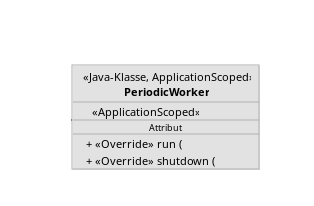
\includegraphics[height=3cm]{graphics/business_internal}
\end{figure}

\classtable{
	\classentry{TrespassListener}{Manages user access to resources, most importantly webpages.}
	\classentry{SessionInformation}{Wraps data saved in the session.}
	\classentry{LifeTimeListener}{Takes care of system start and shutdown operations}
	\classentry{ExceptionHandler}{Handles all Exceptions that leave the business layer by either showing a faces message or an error page.}
	\classentry{Pagination}{}
}
\todo{erklaerung schreiben Pagination}
\subsubsection{de.lasses.control.validation}

\begin{figure}[H]
	\centering
	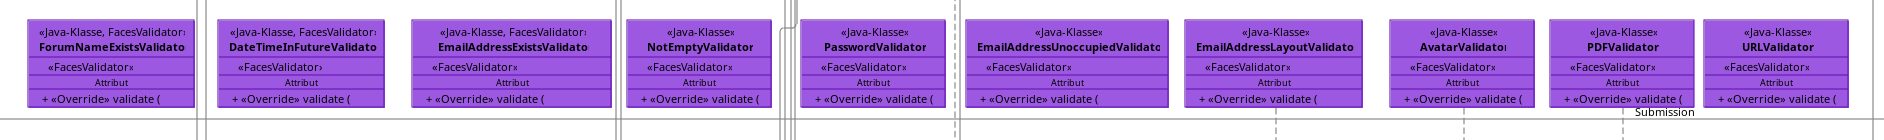
\includegraphics[height=3cm]{graphics/control_validation}
\end{figure}

\classtable{
    \classentry{AvatarValidation}{Validates that a suitable avatar image has been uploaded.}
    \classentry{PDFValidator}{Validates that a suitable PDF file has been uploaded.}
\classentry{EmailAddressLayoutValidation}{Validates that a given String is a valid E-Mail Address.}
\classentry{EmailAdressUnoccupiedValidator}{Validates that a given email is not already in use within the system.}
\classentry{URLValidator}{Validates that a given String is a valid URL.}
	\classentry{PasswordValidator}{Checks if a password meets the minimum requirements for a password.}
	\classentry{NotEmptyValidator}{Checks if a free text imput is empty.}

}

\subsubsection{de.lases.business.service}

Folgende Informationen wurden hier aus Gründen der Übersichtlichkeit aus dem Diagramm ausgespart:
\begin{itemize}
	\item jeder Service benutzt die Transaction Klasse aus dem persistence Package
\end{itemize}

\begin{figure}[H]
	\centering
	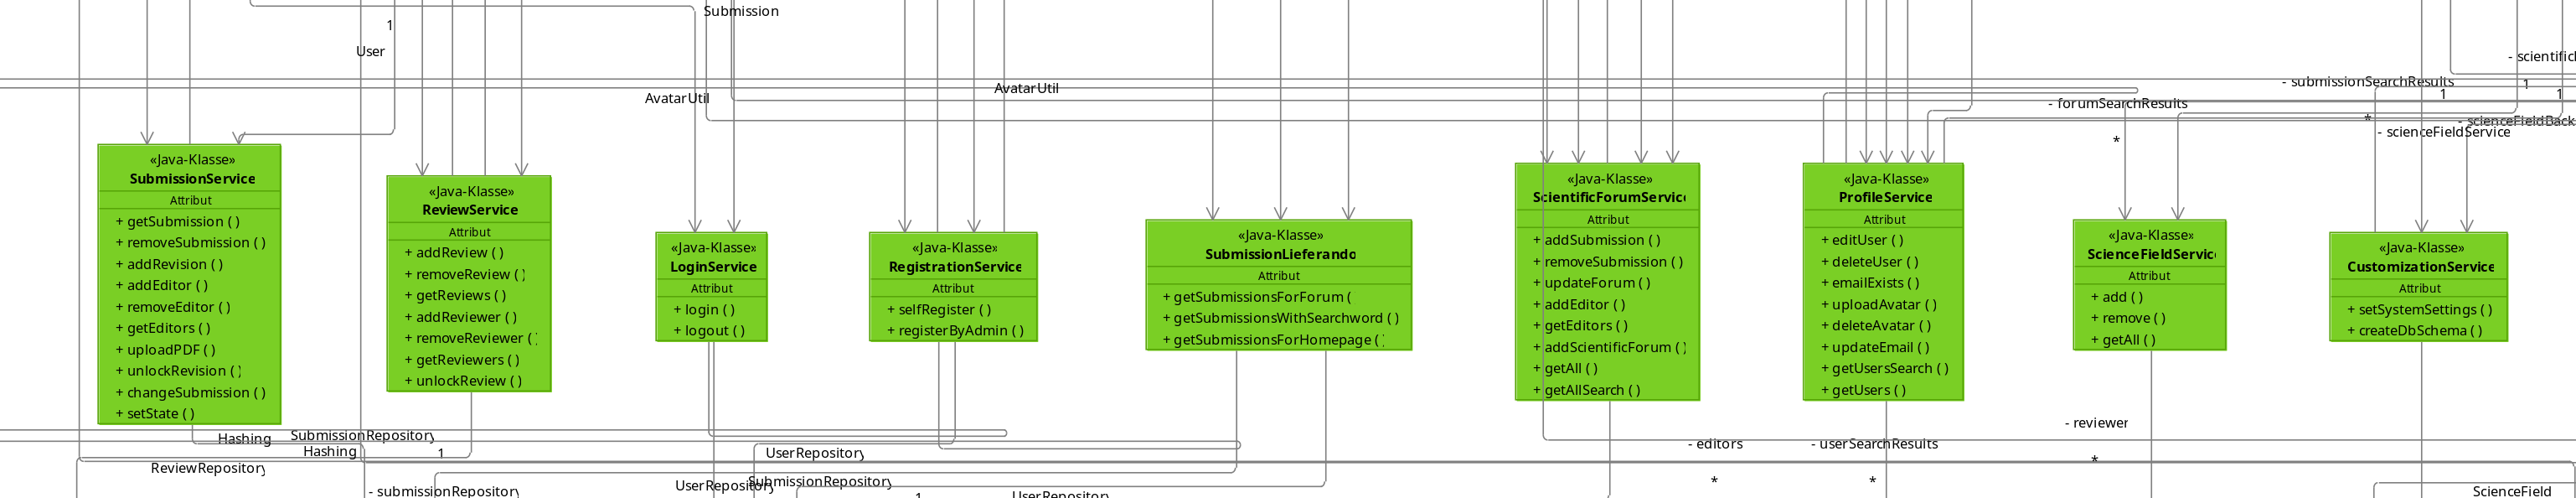
\includegraphics[width=0.9\linewidth]{graphics/business_service}
\end{figure}

\classtable{
	\classentry{CustomizationService}{Provides methods for the manipulation of system settings.}
	\classentry{ScienceFieldService}{Provides methods for adding and removing scientific categories.}
	\classentry{ProfileService}{Provides methods for the manipulation and removal of users.}
	\classentry{ScientificForumService}{Provides methods for the manipulation and creation of scientific forums.}
	\classentry{SubmissionLieferando}{Provides methods for delivering lists of submissions, taking into account
		their filtering, sorting and calling user.}
	\classentry{RegistrationService}{Provides methods for the creation of users.}
	\classentry{LoginService}{Provides methods for the login and logout operations.}
	\classentry{ReviewService}{Provides methods for the delivery, creation and removal of reviews.}
	\classentry{SubmissionService}{Provides methods for the delivery, creation, removal and manipulation of submissions.}
}

\subsubsection{de.lases.business.util}

\begin{figure}[H]
	\centering
	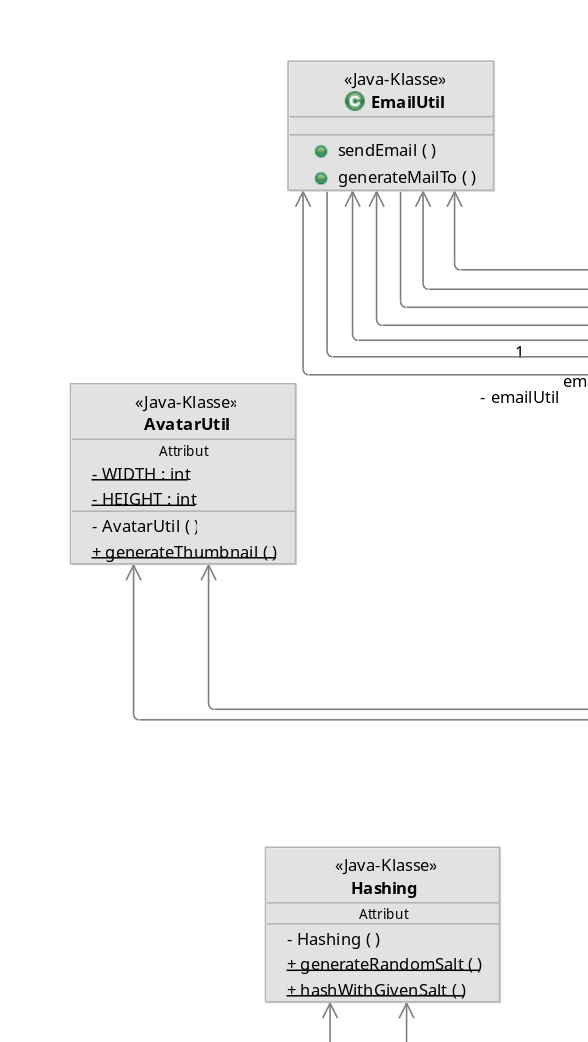
\includegraphics[height=3cm]{graphics/business_util}
\end{figure}

\classtable{
	\classentry{AvatarUtil}{Provides support in the generation of a thumbnail from an image.}
	\classentry{Hashing}{Provides support in the hashing of passwords.}
	\classentry{Lifetime}{Provides a method that should be called on system startup.}
	\classentry{EmailUtil}{Provides support in the sending of emails, creation of mailto links and checking of Email Addresses.}
	\classentry{ConfigPropagator}{The sole purpose of this utility is to make the global configuration available to the control layer.}
}

\subsubsection{de.lases.business.internal}

\begin{figure}[H]
	\centering
	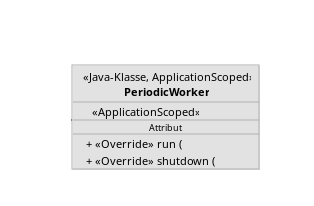
\includegraphics[height=3cm]{graphics/business_internal}
\end{figure}

\classtable{
	\classentry{PeriodicWorker}{Takes care of periodical database cleanup jobs.}
	\classentry{ExceptionQueue}{All exceptions that exit the business layer are put in this queue.}
}

\subsubsection{de.lases.persistence.repository}

Im Folgenden Klassendiagramm gilt:
\begin{itemize}
	\item Jedes Repository ist für genau eine Entität im ER-Diagramm bzw.´ für genau ein DTO zuständig.
	\item Die Methode \emph{getList()} ist jeweils überladen. Falls man eine Liste von Objekten will, die mit einem bestimmten anderen Objekt \emph{a} direkt einer Relationship stehen (siehe ER-Diagramm), dann kann man \emph{a} an die Methode übergeben. Dies ist auch mit mehreren Relationships zugleich möglich.
	\item Spezifische \emph{addObject/removeObject} Methoden sind von der jeweils vorhandenen \emph{change} Methode insofern abzugrenzen, dass sie je Listen von zugeordneten Objekten bearbeiten. Die \emph{change} Methode kann nur Attribute mit Kardinalität 1 bearbeiten. Eine Ausnahme hierbei sind natürlich die \emph{get/set} Methoden für PDFs und Bilder.
\end{itemize}

\begin{figure}[H]
	\centering
	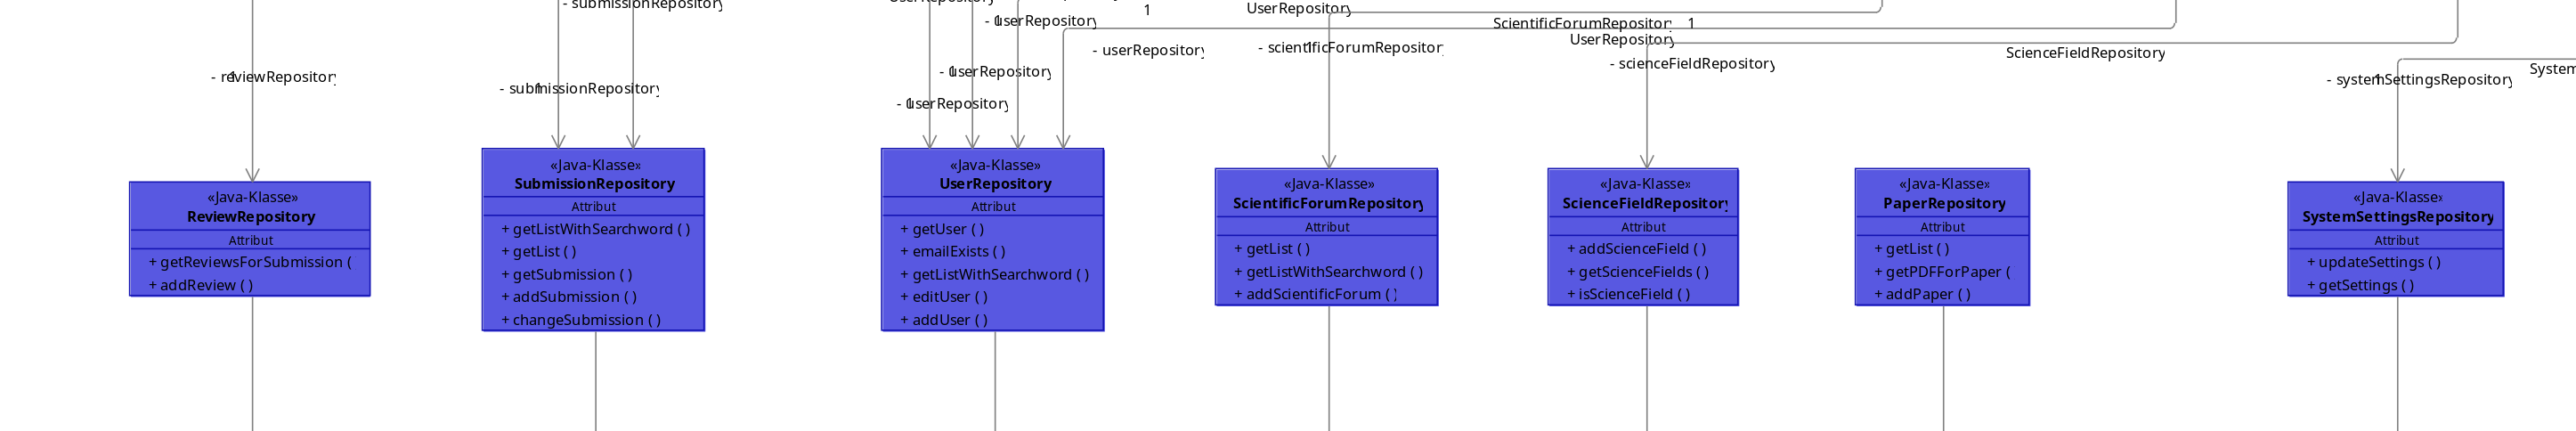
\includegraphics[width=0.9\linewidth]{graphics/persistence_repository}
\end{figure}

\classtable{
    \classentry{PaperRepository}{This repository can get the list of papers for a submission or add new ones.}

    \classentry{ReviewRepository}{This repository can get the reviews for a certain submission and add new ones.}

    \classentry{ScienceFieldRepository}{This repository can get or add new fields of science from/to the database.}

    \classentry{ScientificForumRepository}{This repository can get a list of journals and conferences or add new ones.}

    \classentry{SubmissionRepository}{This repository allows CRUD operations on submissions.}

    \classentry{SystemSettingsRepository}{This repository can read or update the system settings.}

    \classentry{UserRepository}{This repository allows CRUD operations on users.}
}

\subsubsection{de.lases.persistence.util}

\begin{figure}[H]
	\centering
	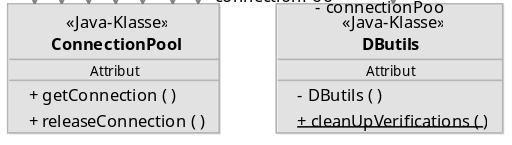
\includegraphics[height=2cm]{graphics/persistence_util}
\end{figure}

\classtable{
    \classentry{ConnectionPool}{Provides and manages connections to the database.}

    \classentry{DButils}{Provides functions for general database services.}
    
    \classentry{EmailSender}{Talks to the SMTP server.}
    
    \classentry{ConfigReader}{Reads the global configuration file from the disk.}
}

\subsubsection{de.lases.persistence.exception}

\begin{figure}[H]
	\centering
	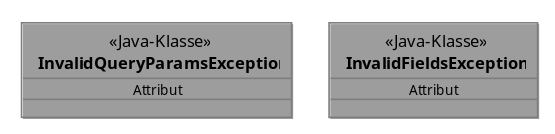
\includegraphics[height=2cm]{graphics/persistence_exception}
\end{figure}

\classtable{
    \classentry{InvalidFieldsException}{Hints at an invalid field in a dto given to the persistence layer.}
    \classentry{InvalidQueryParamsException}{Hints at invalid field in the ResulstListParameters object given to the persistence layer.}
    \classentry{DBConnectionFailedException}{Is thrown when the database connection cannot be established or times out.}
    \classentry{DBConfigurationException}{Is thrown when bad configuration of the database leads to a failure to establish a connection.}
    \classentry{DBQueryFailedException}{Is thrown when a query to the database fails and will probably fail again.}
    \caption{Unchecked Exceptions}
}

\classtable{
	\classentry{EmailAddressExistsException}{Is thrown when the repository tries to save an email-address to the databse that already exists in the database.}
	\classentry{DataNotWrittenException}{Is thrown when the writing of data fails but a retry has a high probability of succeeding.}
	\classentry{DataNotCompleteException}{Is thrown when the reading of data yields an incomplete result but a retry has a high probability of succeeding.}
	\caption{Checked Exceptions}
}



    \section{Bibilotheken}\label{sec:biblithekenn}
    \localauthor{Johann Schicho}

Zur Entwicklung und Verwendung von LasEs werden einige Softwarebibliotheken benötigt. Um keine weiteren Gebühren geltend machen zu müssen, werden nur Bibliotheken mit freien Lizenzen verwendet.

\begin{table}[H]
	\centering
	\begin{tabularx}{\columnwidth}{|l|X|l|}
		\hline
		Name & Beschreibung & Lizenz \\
		\hline\hline
		Mojarra v3.0.1 & Jakarta Server Faces Referenzimplementierung der Eclipse Foundation & EPL v2.0 \\
		\hline
		JBoss Weld v4.0.2.Final & Context and Dependency Injection Referenz Implementierung & Apache 2.0 \\
		\hline
		Primefaces v10.0.0 & UI Komponenten Bibliothek & MIT \\
		\hline
		Bootstrap v5.1.3 & CSS Framework & MIT \\
		\hline
		PostreSQL JDBC v42.3.1 & Datenbank Treiber für PostgreSQL & BSD 2-Clause \\
		\hline
		Jakarta Mail API v2.0.1 & Automatisierte E-Mail Versendung & EPL v2.0 \\
		\hline
		JUnit v5.8.1 & Unit Tests für Java Anwendungen & EPL v2.0 \\
		\hline
		Mockito v4.0.0 & Erzeugung von Mockups zum testen & MIT \\
		\hline
		Selenium v4.0.0 & Automatisierte Browsertests & Apache 2.0 \\
		\hline



	\end{tabularx}
\end{table}

    \section{Konfiguration}\label{sec:konfiguration}
    JSF lässt sich auf verschiedenste Art \& Weisen konfigurieren, wie beispielsweise
mithilfe der \emph{faces-config.xml}.
Die Lases-Anwendung bietet nebenher weitere selbstdefinierte Konfigurationsmöglichkeiten an.
Die Konfigurationsdateien befinden sich im \emph{webapp/WEB-INF/classes} Verzeichnis.
Die Konfigurationsdateien werden intern in \emph{Properties}-Pakete umgewandelt,
wobei jedes \emph{Properties}-Paket eine semantische Aufgabe übernimmt.
So dient beispielsweise die \emph{mail.properties} der Konfiguration des Mailing.
Wenn ein Paket bestimmte \emph{Properties} auslagert,
so landen diese in der Anwendungskonfiguration \emph{config.properties}.
%todo letzten teil kürzen zB letzten satz zu kofig der anw auslagern

\subsection{Konfiguration der Anwendung}
Die Anwendung kann auf einige Weisen personalisiert konfiguriert werden.
Hierzu dient die \emph{config.properties}-Datei,  %todo hyperref
welche zentrale Parameter der Anwendung definiert.

\subsubsection{Konfiguration des Mailings}
Damit die LasEs-Anwendung Mails versenden und Mailto-Links generieren kann
müssen einige Konfigurationsentscheidungen getroffen werden.
Hierzu dient die \emph{mail.properties}-Datei.

\subsubsection{Konfiguration der Datenbank}
Damit die LasEs-Anwendung einen persistenten Datenbankzugriff besitzen kann,
muss dieser konfiguriert werden. Nennenswert sind ebenfalls die
Konfigurationsentscheidungen bezüglich der SSL-Verschlüsselung.
Hierzu dient die \emph{database.properties}-Datei.

\subsubsection{Konfiguration des Logging}
Damit die LasEs-Anwendung aussagekräftige \emph{Log}-Dateien ausgeben kann,
wird der \emph{Logger} konfiguriert.

\subsubsection{Sprachkonfiguration}
Die Dateien, welche die dargestellten \emph{Strings} enthalten befinden sich im
\emph{src/main/ressources}-Verzeichnis.
-bundles / gerüst
-sprach konfiguration -> faces.xml

    \section{Facelets}\label{sec:facelets}
    %% Macros
\newcommand{\ftable}[1]{\begin{longtable}[H]{|m{2cm}|m{3cm}|m{6cm}|m{2.5cm}|}
                            \hline
                            \textbf{ID} & \textbf{Typ} & \textbf{Beschreibung} & \textbf{Sichtbarkeit} \\
                            \hline
                            \hline
                            #1
\end{longtable}
}

\newcommand{\fentry}[4]{#1 & #2 & #3 & #4 \\
\hline}


\localauthor{Stefanie Gürster, Johann Schicho}

Im Folgendem Abschnitt werden Abkürzungen für die verschiedenen Rollen eingeführt:
\textbf{A} steht für Administrator, \textbf{AN} für einen anonymen Nutzer, \textbf{N} für einen angemeldeten Nutzer, \textbf{E} für einen Editor und \textbf{G} steht für einen Gutachter.
Ist eine Funktion für alle Benutzerrollen vorgesehen, so werden diese unter dem Begriff \textbf{Alle} zusammengefasst.

Sind Außerdem keine Labels für Komponenten angegeben, dann sind anstelle dieser Icons (Fontawesome) angedacht.

\subsection{Templates}

\localauthor{Johann Schicho}

% https://stackoverflow.com/questions/4003473/make-an-unbreakable-block-in-tex
% Mit samepage bleiben überschrift und tabelle auf der glechen Seite

\begin{samepage}
    \textbf{navigation.xhtml} ist die Kopfzeile der Webanwendung. Diese bietet die Suchfunktion an und Links zu verschiedenen Listen und dem Profil.
    \nopagebreak

    \ftable{
        \fentry{searchField}{inputText}{Suchleiste}{Alle}

        \fentry{search}{commandButton}{Suche ausführen.}{Alle}

        \fentry{userListLink}{link}{Link zur Übersichtsseite aller Nutzer}{A,E}

        \fentry{forumListLink}{link}{Link zur Übersichtsseite alle Journale und Konferenzen}{Alle}

        \fentry{logoutButton}{commandButton}{Loggt den Nutzer aus dem System aus und leitet zur Loginseite weiter}{Alle}

        \fentry{profileLink}{link}{Link zur Profilübersicht}{N}

    }
\end{samepage}

\begin{samepage}
    \textbf{main.xhtml} ist das Template, welches den Inhalt der Seiten zwischen Kopf- und Fußzeile einbettet.

    \ftable{
        \fentry{navigationBar}{include}{Kopfzeile}{Alle}

        \fentry{mainContent}{insert}{Seiteninhalt}{Alle}

        \fentry{footerBar}{include}{Fußzeile}{Alle}

        \fentry{toolBar}{include}{Seitenleiste}{A,E}

    }
\end{samepage}

\begin{samepage}
    \textbf{footer.xhtml} ist die Fußzeile der Webanwendung und für alle sichtbar.
    \nopagebreak

    \ftable{
        \fentry{imprintLink}{link}{Link zur Seite des Impressums}{Alle}

        \fentry{language}{outputText}{Anzeige der eingestellten Sprache.}{Alle}

    }
\end{samepage}

\begin{samepage}
    \textbf{toolbar.xhtml} ist die Seitenleiste für Editoren und Administratoren auf der Einreichungsübersicht. Hier wird die Einreichung verwaltet.
    \nopagebreak

    \ftable{
        \fentry{reviewerLabel}{outputLabel}{Label für Gutachterangabe.}{A,E}

        \fentry{addReviewerField}{inputText}{Eingabefeld zur Angabe einer E-Mailadresse}{A,E}

        \fentry{deadlineReviewer}{outputLabel}{Label für Deadline.}{A,E}

        \fentry{addDeadlineReviewer}{inputText}{Eingabefeld zur Angabe einer Deadline.}{A,E}

        \fentry{addReviewerBtn}{commandButton}{Knopf zum hinzufügen des Gutachters}{A,E}

        \fentry{reviewerTable}{dataTable}{Liste der Gutachter}{A,E}

        \fentry{removeReviewer}{commandButton}{Entferne einen bestimmten Gutachter}{A,E}

        \fentry{editorLabel}{outputLabel}{Label für Editorauswahl.}{A,E}

        \fentry{selectEditor}{selectOneMenu}{Auswahländerung des verwaltenden Editors}{A,E}

        \fentry{saveEditor}{commandButton}{Speichern der Änderung}{A,E}

        \fentry{deadlineRevision}{outputLabel}{Label für Deadline.}{A,E}

        \fentry{revisionDeadline}{inputText}{Eingabe zur Angabe einer Deadline.}{A,E}

        \fentry{requireRevisionBtn}{commandButton}{Fordert den Einreicher auf, seine Einreichung zu überarbeiten}{A,E}

        \fentry{acceptSubmissionBtn}{commandButton}{Akzeptiere die Einreichung}{A,E}

        \fentry{rejectSubmissionBtn}{commandButton}{Lehne die Einreichung ab}{A,E}

    }
\end{samepage}

\localauthor{Stefanie Gürster}

\begin{samepage}
    \textbf{listPagination.xhtml} ist eine Composite Component zur Paginierung von Listen.
    \emph{listPagination.xhtml} wird in jedem Footer einer Tabelle eingebunden.
    \todo{Beschreibung von ListPagination verändern.}
    \nopagebreak

    \ftable{
        \fentry{back}{commandButton}{Laden der vorherigen Seite der Liste.}{Alle}

        \fentry{next}{commandButton}{Laden der nächsten Seite der Liste.}{Alle}

        \fentry{page}{selectOneMenu}{Laden einer bestimmten Seite}{Alle}
    }
\end{samepage}

\subsection{Seiten}

\localauthor{Stefanie Gürster}

\begin{samepage}
    \textbf{initialConfig.xhtml} Auf dieser Seite landet man beim ersten Systemstart. Sie ist nur für Administratoren zugänglich.
    Hier kann der Administrator die Datenbankschemata erstellen lassen.
    \nopagebreak

    \ftable{
        \fentry{dbConnectionState}{outputText}{Information über die Verbindung mit der Datenbank}{A}

        \fentry{createDbBtn}{commandButton}{Erstellt die Datenbankschemata}{A}
    }
\end{samepage}

\begin{samepage}
    \textbf{welcome.xhtml} Auf der Login- bzw. Welcome-Seite wird \emph{LasEs} vorgestellt.
    Zusätzlich gibt es ein Login-Formular zur Anmeldung im System.
    Für nicht registrierte Nutzer wird man über einen gegebenen Link zu \emph{registration.xhtml} weitergeleitet.
    \nopagebreak

    \ftable{

        \fentry{welcomeHeading}{outputText}{Überschrift der Welcomepage.}{Alle}

        \fentry{welcomeText}{outputText}{Bewerben der Applikation mithilfe einer Kurzbeschreibung.}{Alle}

        \fentry{email}{inputText}{Textfeld für E-Mail Eingabe.}{Alle}

        \fentry{password}{inputSecret}{Textfeld für Passwort Eingabe.}{Alle}

        \fentry{login}{commandButton}{Ausführen des Login-Prozesses.}{Alle}

        \fentry{register}{link}{Weiterleitung zur Registrierung.}{Alle}

    }
\end{samepage}

\begin{samepage}
    \textbf{registration.xhtml} Seite zur Registrierung anonymer Nutzer.
    \nopagebreak

    \ftable{
        \fentry{titelLabel}{outputLabel}{Label für Titel.}{AN}

        \fentry{title}{inputText}{Angabe eines Titels.}{AN}

        \fentry{firstNameLabel}{outputLabel}{Label für Vorname.}{AN}

        \fentry{firstName}{inputText}{Angabe des Vornamens.}{AN}

        \fentry{nameLabel}{outputLabel}{Label für Nachname.}{AN}

        \fentry{name}{inputText}{Angabe des Nachnamen.}{AN}

        \fentry{passwordLabel}{outputLabel}{Label für Passwort.}{AN}

        \fentry{password}{inputSecret}{Angabe eines Passwortes.}{AN}

        \fentry{emailLabel}{outputLabel}{Label für E-Mail.}{AN}

        \fentry{email}{inputText}{Angabe einer validen E-Mail.}{AN}

        \fentry{register}{commandButton}{Ausführen des Registrations-Prozesses.}{AN}

        \fentry{welcomepage}{link}{Weiterleitung zur Login Seite.}{AN}
    }
\end{samepage}

\begin{samepage}
    \textbf{verification.xhtml} Wird bei erfolgreicher Verifikation der E-Mail angezeigt.
    \nopagebreak

    \ftable{

        \fentry{successText}{outputText}{Text zur erfolgreichen Verifizierung der E-Mail}{Alle}

        \fentry{countdown}{timer}{Timer bis zur Weiterleitung auf die Homepage.}{Alle}

    }
\end{samepage}

\textbf{homepage.xhtml}\label{flt:homepage} Startseite die den Überblick über alle Einreichungen beinhaltet.

\begin{samepage}
    \ftable{
        \fentry{yourSubmission}{commandLink}{Reiter zum Anzeigen der eigenen Einreichungen.}{Alle}

        \fentry{yourReviews}{commandLink}{Reiter zum Anzeigen der zu begutachtenden Einreichungen}{G}

        \fentry{editorialOverview}{commandLink}{Reiter zum Anzeigen aller Einreichungen, welche man editiert.}{E}

        \fentry{filterLabel}{outputLabel}{Label für Filter}{Alle}

        \fentry{stateLabel}{outputLabel}{Label für Filter vom Status der Einreichung}{Alle}

        \fentry{stateSelect}{selectOneMenu}{Filtern des Status von Einreichungen}{Alle}

        \fentry{dateLabelBefore}{outputLabel}{Label für Filter nach einem Datum.}{Alle}

        \fentry{dateBefore}{inputText}{Eingabe eines \emph{spätestens} Datum}{Alle}

        \fentry{dateLabelAfter}{outputLabel}{Label für Filter vor einem Datum.}{Alle}

        \fentry{dateAfter}{inputText}{Eingabe eines \emph{frühestens} Datum}{Alle}

        \fentry{dateUp}{commandButton}{Einreichungen werden dem Datum nach aufsteigend angezeigt.}{Alle}

        \fentry{dateDown}{commandButton}{Einreichungen werden dem Datum nach absteigend angezeigt.}{Alle}

        \fentry{searchLabel}{outputLabel}{Label für Suche.}{Alle}

        \fentry{search}{inputText}{Durchsuchen der Tabellen mit Matching-Words.}{Alle}

        \fentry{apply}{commandButton}{Wende Filtereinstellungen an.}{Alle}

        \fentry{submissionTable}{dataTable}{Liste aller eignen Einreichungen.}{Alle}

        \fentry{reviewTable}{dataTable}{Liste aller Gutachten.}{G}

        \fentry{editorTable}{dataTable}{Liste aller Einreichungen für einen Editor.}{E}

        \fentry{pagination}{listPagination}{Jede Tabelle enthält eine Paginierung.}{Alle}
    }
\end{samepage}

\begin{samepage}
    Die einzelnen Tabellen \emph{submissionTable}, \emph{reviewTable} und \emph{editorTable} sind nach den gleichen Punkten gegliedert: Titel des Papers, Datum und Status der Einreichung und Name des zugehörigen Forums.

    \ftable{
        \fentry{title}{Link}{Titel des Papers und Weiterleitung zur Einreichung}{Alle}

        \fentry{date}{outputText}{Datum der Einreichung.}{Alle}

        \fentry{state}{outputText}{Status der Einreichung.}{Alle}

        \fentry{forum}{Link}{Name des zugehörigen Forums und Weiterleitung zum Forum.}{Alle}
    }
\end{samepage}

\begin{samepage}

    \textbf{submission.xhtml} ist die Übersichtsseite einer Abgabe.
    Hier werden alle mit der Einreichung verbundenen Aktivitäten abgebildet.
    Für den \textbf{Editor} und den \textbf{Administrator} wird zusätzlich eine \emph{toolbar.xhtml} eingebunden.
    \nopagebreak

    \ftable{
        \fentry{title}{outputText}{Titel des Papers.}{Alle}

        \fentry{forumLabel}{outputLabel}{Label für ein Forum.}{Alle}

        \fentry{forum}{Link}{Name des Forums und Weiterleitung zur Forumsübersicht.}{Alle}

        \fentry{authorLabel}{outputLabel}{Label für Autor.}{Alle}

        \fentry{author}{Link}{Name des Autors und Weiterleitung zum Profil.}{Alle}

        \fentry{coAuthorLabel}{outputLabel}{Namen der Co-Autoren.}{Alle}

        \fentry{emailLabel}{outputLabel}{Label für E-Mail-Adressen der Co-Authoren.}{Alle}

        \fentry{email}{Link}{E-Mail-Adressen der Co-Authoren und Mailto-Link.}{Alle}

        \fentry{filterLabel}{outputLabel}{Label für Filter}{Alle}

        \fentry{dateLabel}{outputLabel}{Label für Filter von Datum.}{Alle}

        \fentry{dateUp}{commandButton}{Einreichungen werden aufsteigend angezeigt.}{Alle}

        \fentry{dateDown}{commandButton}{Einreichungen werden absteigend angezeigt.}{Alle}

        \fentry{reviewStateLabel}{outputLabel}{Label für Filtern der Gutachtenfreischaltung.}{E,A}

        \fentry{all}{checkbox}{Anzeigen aller Gutachten.}{E,A,G}

        \fentry{allLabel}{outputLabel}{Label für all.}{E,A,G}

        \fentry{locked}{checkbox}{Anzeigen nicht freigeschalteter Gutachten.}{E,A,G}

        \fentry{lockedLabel}{outputLabel}{Label für locked.}{E,A,G}

        \fentry{unlocked}{checkbox}{Anzeigen freigeschalteter Gutachten.}{E,A,G}

        \fentry{unlockedLabel}{outputLabel}{Label für unlocked.}{E,A,G}

        \fentry{reviewSubmitLabel}{outputLabel}{Label für Filter von eingereichten Gutachten.}{E,A}

        \fentry{submitted}{checkbox}{Anzeigen aller abgegebenen Gutachten.}{E,A}

        \fentry{submittedLabel}{outputLabel}{Label für submitted.}{E,A}

        \fentry{notSubmitted}{checkbox}{Anzeigen noch nicht abgegebener Gutachten.}{E,A}

        \fentry{notSubmittedLabel}{outputLabel}{Label für notSubmitted.}{E,A}

        \fentry{versionLabel}{outputLabel}{Label für Versionsfilter.}{Alle}

        \fentry{version}{selectOneMenu}{Auswahl der Versionsnummern}{Alle}

        \fentry{reviewerLabel}{outputLabel}{Label für Reviewerfilter.}{Alle}

        \fentry{reviewer}{selectOneMenu}{Auswahl eines bestimmten Gutachters.}{E,A}

        \fentry{recommendationLabel}{outputLabel}{Label für Empfehlungen.}{E,A,G}

        \fentry{recommendation}{selectOneMenu}{Auswahl der Art von Empfehlungen.}{E,A,G}

        \fentry{searchLabel}{outputLabel}{Label für Suche.}{Alle}

        \fentry{search}{inputText}{Durchsuchen der Tabelle mit Matching-Words.}{Alle}

        \fentry{apply}{commandButton}{Wende Filtereinstellungen an.}{Alle}

        \fentry{submissionTable}{dataTable}{Liste aller Versionen}{Alle}

        \fentry{reviewTable}{dataTable}{Liste aller/der eigenen Gutachten.}{E,A,G}

        \fentry{pagination}{listPagination}{Jede Tabelle enthält eine Paginierung.}{Alle}
    }

    \emph{submissionTable} enthält die Spalten: Version, Datum, Deadline, Status und Download.
    Die Elemente der Liste, der unterschiedlichen Versionen der Einrichtung, sieht wie folgt aus:

    \ftable{
        \fentry{version}{outputText}{Versionsnummer der Einreichung}{Alle}

        \fentry{date}{outputText}{Datum der Einreichung}{Alle}

        \fentry{deadline}{outputText}{Deadline der Revision}{Alle}

        \fentry{state}{radioButton}{Status der Einreichung}{Alle}

        \fentry{pdf}{inputFile}{Download der Einreichung}{Alle}
    }

    \emph{reviewTable} enthält die Spalten: Version, Gutachter, Datum, Deadline, Status, Empfehlung, Kommentar und Download.
    Die Elemente der Liste von Gutachten ist wie folgt:

    \ftable{
        \fentry{version}{outputText}{Versionsnummer des Gutachtens.}{E,A,G}

        \fentry{reviewer}{outputText}{Namen des Gutachters.}{E,A,G}

        \fentry{date}{outputText}{Datum des Gutachtens.}{E,A,G}

        \fentry{deadline}{outputText}{Deadline des Gutachtens.}{E,A,G}

        \fentry{state}{commandButton}{Freigabe des Gutachtens}{E,A}

        \fentry{stateText}{outputText}{Freigabestatus des Gutachtens}{G}

        \fentry{recomendation}{checkbox}{Empfehlung eines Gutachters}{E,A,G}

        \fentry{comment}{outputText}{Kommentar des Gutachters.}{E,A,G}

        \fentry{pdf}{inputFile}{Download der Einreichung}{E,A,G}
    }
\end{samepage}

\begin{samepage}
    \textbf{newSubmission.xhtml} Hier können neue Paper eingereicht werden.
    \nopagebreak

    \ftable{
        \fentry{subNameLabel}{outputLabel}{Label für Papertitel.}{N
        }
        \fentry{submissionName}{inputText}{Name des abzugebenden Papers.}{N}

        \fentry{forumLabel}{outputLabel}{Label für Name des Forums.}{N}

        \fentry{forumName}{inputText}{Name des Forums, bei welchem abgegeben wird.}{N }

        \fentry{editorLabel}{outputLabel}{Label für Editor.}{N}

        \fentry{editorSearch}{selectOneMenu}{Angabe eines Editors}{N}

        \fentry{pfdUpload}{inputFile}{Angabe der Abgabedatei.}{N}

        \fentry{titleLabel}{outputLabel}{Label für Titel}{N}

        \fentry{titel}{inputText}{Angabe eines Titels.}{N}

        \fentry{coAuthorLabel}{outputLabel}{Label für Co-Autor.}{N}

        \fentry{coAuthorFirstLabel}{outputLabel}{Label für Vorname des Co-Autors.}{N}

        \fentry{coAuthorFirstName}{inputText}{Angabe des Vornamen eines Co-Autors.}{N}

        \fentry{coAuthorLastLabel}{outputLabel}{Label für Nachname des Co-Autors.}{N}

        \fentry{coAuthorLastName}{inputText}{Angabe des Namen eines Co-Autors.}{N}

        \fentry{coAuthorEmailLabel}{outputLabel}{Label für E-Mail des Co-Autors.}{N}

        \fentry{coAuthorEMail}{inputText}{Angabe der E-Mail eines Co-Autors.}{N}

        \fentry{submitCoAuthor}{commandButton}{Ausgabe des Co-Autors in einer Liste.}{N}

        \fentry{coAuthorList}{outputText}{Anzeige aller Co-Authoren in einer Liste.}{N}

        \fentry{deleteCoAuthor}{commandButton}{Löschen des zugehörigen Co-Authors.}{N}

        \fentry{submit}{commandButton}{Ausführen des Abgabe-Prozesses.}{N}
    }
\end{samepage}

\begin{samepage}
    \textbf{newReview.xhtml} Möchte ein Gutachter eines Papers seine Beurteilung abgeben, so ist dies auf dieser Seite möglich.
    \nopagebreak

    \ftable{
        \fentry{versionLabel}{outputLabel}{Label für Versionsnummer}{G,A}

        \fentry{versionNumber}{outputText}{Versionsnummer des eingereichten Papers, zu welchem der Gutachter ein Gutachten abgeben kann.}{G,A}

        \fentry{recommendationLabel}{outputLabel}{Label für eine Empfehlung.}{G,A}

        \fentry{recommendation}{checkbox}{Empfehlung des Gutachters ein Paper zu akzeptieren.}{G,A}

        \fentry{commentLabel}{outputLabel}{Label für einen Kommentar}{G,A}

        \fentry{comment}{inputTextarea}{Kommentar eines Gutachters}{G,A}

        \fentry{pdfLabel}{outputLabel}{Label für Datei}{G,A}

        \fentry{reviewPdf}{inputFile}{Einzureichendes Gutachten.}{G,A}
    }
\end{samepage}


\begin{samepage}
    \textbf{resultList.xhtml} zeigt alle Ergebnisse einer Suche an.
    \nopagebreak

    Wird nach den eigenen Einreichungen, nach denen die man begutachtet oder nach Einreichungen in eingener editorialen Verantwortung gesucht, so erscheinen die Listen im gleiche Schema wie auch auf \hyperref[flt:homepage]{der Homepage}.
    Ergibt die Suche eine Liste von User, so wird diese wie in \hyperref[flt:userList]{der Userliste} für den Administrator und dem Editor angezeigt.
    Ist das Ziel der Suche, wissenschaftliche Foren zu finden so erhält man bei passender Eingabe eine Liste im selben Format wie diejenige auf der \hyperref[flt:forumList]{Seite der Forumsliste.}
\end{samepage}


\begin{samepage}
    \localauthor{Johann Schicho}\nopagebreak

    \textbf{scientificForumList.xhtml} \label{flt:forumList} Hier erhalten die Nutzer eine Übersicht über alle wissenschaftliche Foren.\nopagebreak

    \ftable{

        \fentry{filterLabel}{outputLabel}{Label für Filter}{Alle}

        \fentry{scFieldsLabel}{outputLabel}{Label für Filter der Themengebiete}{Alle}

        \fentry{scFieldSelect}{selectOneMenu}{Filtern der Themengebiete der Foren}{Alle}

        \fentry{deadlineLabel}{outputLabel}{Label für Filtern nach Deadlines (Abgelaufen/Zukunft)}{Alle}

        \fentry{deadlineSelect}{selectOneMenu}{Filtern der nach Deadlines}{Alle}

        \fentry{dateLabelBefore}{outputLabel}{Label für Deadline nach einem Datum.}{Alle}

        \fentry{dateBefore}{inputText}{Eingabe eines \emph{spätestens} Datum}{Alle}

        \fentry{dateLabelAfter}{outputLabel}{Label für Deadline vor einem Datum.}{Alle}

        \fentry{dateAfter}{inputText}{Eingabe eines \emph{frühestens} Datum}{Alle}

        \fentry{searchLabel}{outputLabel}{Label für Suche.}{Alle}

        \fentry{search}{inputText}{Durchsuchen der Tabelle mit Matching-Words.}{Alle}

        \fentry{apply}{commandButton}{Wende Filtereinstellungen an.}{Alle}

        \fentry{nameUp}{commandButton}{Einreichungen werden aufsteigend nach Namen angezeigt.}{Alle}

        \fentry{nameDown}{commandButton}{Einreichungen werden absteigend nach Namen angezeigt.}{E,A}

        \fentry{deadlineUp}{commandButton}{Einreichungen werden aufsteigend nach Deadline angezeigt.}{Alle}

        \fentry{deadlineDown}{commandButton}{Einreichungen werden absteigend nach Deadline angezeigt.}{Alle}

        \fentry{forumsTable}{dataTable}{Liste aller Foren im System.}{Alle}

        \fentry{pagination}{listPagination}{Die Tabelle enthält eine Paginierung.}{Alle}
    }
\end{samepage}

\begin{samepage}
    \localauthor{Stefanie Gürster}\nopagebreak

    Die Liste aller Foren im System wird in folgende Bereiche unterteilt: Name des Forums, Deadline und Kategorie.
    Dabei beinhaltet jede Zeile dieser Liste folgende Elemente:

    \ftable{
        \fentry{name}{link}{Name des Forums.}{Alle}

        \fentry{deadline}{outputText}{Abgabefrist des jeweiligen Forums.}{Alle}

        \fentry{scienceField}{outputText}{Kategorie des Forums.}{Alle}
    }
\end{samepage}


\begin{samepage}

    \textbf{profile.xhtml} Die Profilseite eines angemeldeten Nutzers ist nur vom Nutzer selbst und vom Administrator editierbar.
    Ein Editor besitzt nur Leserechte. Alle zuvor gespeicherten Angaben werden in den jeweiligen Feldern angezeigt.
    \nopagebreak

    \ftable{

        \fentry{avatar}{graphicImage}{Aktueller Avatar.}{N,A,E}

        \fentry{newAvatar}{inputFile}{Hochladen eines neuen Avatars.}{N,A,E}

        \fentry{deleteAvatar}{commandButton}{Löschen des Avatars.}{N,A,E}

        \fentry{roleLabel}{outputLabel}{Label für Rolle.}{N,A,E}

        \fentry{role}{outputText}{Angabe der Rolle eines Nutzers}{N,A,E}

        \fentry{isAdminLabel}{outputLabel}{Label für Adminrolle.}{A}

        \fentry{isAdmin}{checkbox}{Zuteilung der Rolle des Administrators.}{A}

        \fentry{titleLabel}{outputLabel}{Label für Titel}{N,A,E}

        \fentry{title}{inputText}{Titel des Nutzenden.}{N,A,E}

        \fentry{firstNameLabel}{outputLabel}{Label für Vorname}{N,A,E}

        \fentry{firstName}{inputText}{Vorname des Nutzenden.}{N,A,E}

        \fentry{nameLabel}{outputLabel}{Label für Nachname}{N,A,E}

        \fentry{name}{inputText}{Nachname des Nutzenden.}{N,A,E}

        \fentry{passwordLabel}{outputLabel}{Label für Passwort.}{N,A}

        \fentry{password}{inputSecret}{Leeres Eingabefeld für ein neues Passwort.}{N,A}

        \fentry{emailLabel}{outputLabel}{Label für E-Mail.}{N,A,E}

        \fentry{email}{inputText}{E-Mail des Nutzenden.}{N,A,E}

        \fentry{submissionNumberLabel}{outputLabel}{Label für Anzahl von Einreichungen.}{N,A,E}

        \fentry{submissionNumber}{outputText}{Anzahl der eigenen Einreichungen}{N,A,E}

        \fentry{employerLabel}{outputLabel}{Label für Arbeitgeber}{N,A,E}

        \fentry{employer}{inputText}{Angabe des Arbeitgebers}{N,A,E}

        \fentry{sciencFieldLabel}{outputLabel}{Label für Fachgebiet}{N,A,E}

        \fentry{scieneField}{outputText}{Liste aller Fachgebiete}{N,A,E}

        \fentry{addScienceField}{inputText}{Spezialgebiete des Nutzers}{N,A,E}

        \fentry{addFieldButton}{commandButton}{Füge Fachgebiet zur Liste hinzu.}{N,A,E}

        \fentry{dateOfBirthLabel}{outputLabel}{Label für Geburtstag.}{N,A}

        \fentry{dateOfBirth}{inputText}{Angabe des Geburtstages}{N,A}

        \fentry{save}{commandButton}{Daten werden persistiert.}{N,A,E}

        \fentry{delete}{commandButton}{Nutzer und alle damit verbundenen Daten werden gelöscht.}{N,A,E}
    }
\end{samepage}

Sollte ein Administrator einem anderen Nutzer die Rolle des Administrators zuweisen oder entziehen, so erscheint beim Auslösen des Save-Buttons ein Popup-Dialog.
In diesem Fenster wird der Administrator angewiesen, die Änderung mit seinem Passwort zu bestätigen.

\ftable{

    \fentry{password}{inputSecret}{Angabe eines Passworts.}{A}

    \fentry{reference}{outputText}{Hinweis zur Veränderung der Adminrolle.}{A}

    \fentry{abort}{commandButton}{Abbruch der Änderung.}{A}

    \fentry{save}{commandButton}{Speichern aller Änderungen.}{A}

}

\begin{samepage}
    \textbf{errorPage.xhtml} Auf diese Seite wird navigiert, wenn auf eine nicht existierende URL oder auf eine URL zugegriffen wird, auf die man keine Zugriffsrechte hat.
    \nopagebreak

    \ftable{

        \fentry{errorMessage}{outputText}{Anzeige einer Fehlermeldung.}{Alle}

    }
\end{samepage}


\begin{samepage}
    \localauthor{Johann Schicho} \nopagebreak

    \textbf{userList.xhtml} \label{flt:userList} Editoren und Administratoren erhalten hier einen Überblick über alle Nutzer. Die Seiten sind paginiert.
    \nopagebreak

    \ftable{

        \fentry{filterLabel}{outputLabel}{Label für Filter}{E,A}

        \fentry{roleLabel}{outputLabel}{Label für Filter Rolle des Nutzers}{E,A}

        \fentry{roleSelect}{selectOneMenu}{Filtern der Rolle des Nutzers}{E,A}

        \fentry{searchLabel}{outputLabel}{Label für Suche.}{Alle}

        \fentry{search}{inputText}{Durchsuchen der Tabelle mit Matching-Words.}{Alle}

        \fentry{apply}{commandButton}{Wende Filtereinstellungen an.}{E,A}

        \fentry{nameUp}{commandButton}{Nutzer werden nach Namen aufsteigend angezeigt.}{E,A}

        \fentry{nameDown}{commandButton}{Nutzer werden absteigend nach Namen angezeigt.}{E,A}

        \fentry{roleUp}{commandButton}{Nutzer werden nach Rolle aufsteigend angezeigt.}{E,A}

        \fentry{roleDown}{commandButton}{Nutzer werden absteigend nach Rolle angezeigt.}{E,A}

        \fentry{roleLabel}{outputLabel}{Label für Rolle}{E,A}

        \fentry{role}{selectOneMenu}{Auswahl der Rollen.}{E,A}

        \fentry{userTable}{dataTable}{Liste aller Nutzer im System.}{E,A}

        \fentry{pagination}{listPagination}{Die Tabelle enthält eine Paginierung.}{E,A}
    }
\end{samepage}

\begin{samepage}
    \localauthor{Stefanie Gürster}\nopagebreak

    Für die Benutzerliste sind die folgenden Elemente vorgesehen, wobei diese in die Bereiche: Nutzerrolle, Name, E-Mail-Adresse, Arbeitgeber und Fachgebiete aufgegliedert ist.

    \ftable{
        \fentry{role}{outputText}{Rolle des Nutzers}{E,A}

        \fentry{name}{link}{Name des Nutzers.}{E,A}

        \fentry{email}{link}{E-Mail-Adresse des Nutzers.}{E,A}

        \fentry{employee}{outputText}{Arbeitgeber des Nutzers.}{E,A}

        \fentry{scienceField}{outputText}{Fachgebiete des Nutzers.}{E,A}
    }
\end{samepage}

\begin{samepage}

    \textbf{newUser.xhtml} Der Administrator kann hier einen neuen Nutzer anlegen.
    \nopagebreak

    \ftable{
        \fentry{passwordLabel}{outputLabel}{Label für Passwort.}{A}

        \fentry{password}{inputSecret}{Angabe des Passworts.}{A}

        \fentry{firstLabel}{outputLabel}{Label für Vorname.}{A}

        \fentry{firstName}{inputText}{Angabe des Vornamen.}{A}

        \fentry{nameLabel}{outputLabel}{Label für Nachname}{A}

        \fentry{name}{inputText}{Angabe des Nachnamen.}{A}

        \fentry{titleLabel}{outputLabel}{Label für Titel}{A}

        \fentry{titel}{inputText}{Angabe eines Titels.}{A}

        \fentry{emailLabel}{outputLabel}{Label für E-Mail.}{A}

        \fentry{email}{inputText}{Angabe einer E-Mail-Adresse.}{A}

        \fentry{isAdminLabel}{outputLabel}{Label für Adminrolle.}{A}

        \fentry{isAdmin}{checkbox}{Zuordnung einer Administratorenrolle.}{A}

        \fentry{abort}{commandButton}{Abbruch des Vorgangs: Nutzererstellen.}{A}

        \fentry{save}{commandButton}{Speichern des neuen Nutzers.}{A}

    }
\end{samepage}

\begin{samepage}
    \textbf{administration.xhtml} Hier kann ein Administrator Konfigurationen vornehmen.
    \nopagebreak

    \ftable{

        \fentry{themeHeading}{outputText}{Überschrift für Farbthemes.}{A}

        \fentry{orangeTheme}{outputLabel}{Standart Theme der Applikation.}{A}

        \fentry{orange}{radioButton}{Auswahl des Standart Themes.}{A}

        \fentry{darkTheme}{outputLabel}{Dark Theme der Applikation.}{A}

        \fentry{dark}{radioButton}{Auswahl des Dark Themes.}{A}

        \fentry{blueTheme}{outputLabel}{Blue Theme der Applikation}{A}

        \fentry{blue}{radioButton}{Auswahl des Blue Themes.}{A}

        \fentry{greenTheme}{outputLabel}{Green Theme der Applikation.}{A}

        \fentry{green}{radioButton}{Auswahl des Green Themes.}{A}

        \fentry{logoHeading}{outputText}{Überschrift für Logo-Bereich.}{A}

        \fentry{logo}{graphicImage}{Logo des Systems.}{A}

        \fentry{changeLogo}{inputFile}{Hochladen eines neuen Logos.}{A}

        \fentry{institutionHeading}{outputText}{Überschrift für Einstellungen der Einrichtung.}{A}

        \fentry{institution}{inputText}{Angabe des Namens der Einrichtung.}{A}

        \fentry{imprint}{inputTextArea}{Angabe des Impressums der Einrichtung.}{A}

        \fentry{abort}{commandButton}{Abbruch des Änderungsvorgangs.}{A }

        \fentry{save}{commandButton}{Speichern der Änderungen.}{A}

        \fentry{newUser}{link}{Weiterleitung zu \emph{newUser.xhtml}.}{A}

        \fentry{newScientificForum}{link}{Weiterleitung zu \emph{newScientificForum.xhtml}.}{A}
    }
\end{samepage}

\begin{samepage}
    \textbf{newScientificForum.xhtml} Auf der Seite zum Erstellen eines wissenschaftlichen Forums kann ein Administrator dessen wesentlichen Daten festlegen.
    \nopagebreak

    \ftable{

        \fentry{forumName}{inputText}{Angabe des Name des Forums.}{A}

        \fentry{fName}{outputLabel}{Label Name des Forums.}{A}

        \fentry{editorLabel}{outputLabel}{Label für Editorauswahl.}{A}

        \fentry{emailEditor}{inputText}{Angabe der E-Mail-Adresse eines Editor.}{A}

        \fentry{emailEditorLabel}{outputLabel}{Label für E-Mail-Adresse eines Editors.}{A}

        \fentry{addEditor}{commandButton}{Hinzufügen eines Editors in eine Liste.}{A}

        \fentry{deleteEditor}{commandButton}{Löschen des zugehörigen Editors von der Liste.}{A}

        \fentry{deadline}{inputText}{Hinzufügen einer Deadline des Forums.}{A}

        \fentry{deadlineLabel}{outputLabel}{Label für Deadline des Forums.}{A}

        \fentry{description}{inputTextArea}{Angabe einer Kurzbeschreibung.}{A}

        \fentry{descriptionLabel}{outputLabel}{Label für Kurzbeschreibung.}{A}

        \fentry{url}{inputText}{Link zur Konferenz oder zum Journal.}{A}

        \fentry{urlLabel}{outputLabel}{Label für URL des Forums.}{A}

        \fentry{instructionLabel}{outputLabel}{Label für Anleitung}{A}

        \fentry{reviewInstructions}{inputTextArea}{Angabe einer Anleitung für eine Begutachtung.}{A}

        \fentry{scienceFieldLabel}{outputLabel}{Label für Fachgebiete}{A}

        \fentry{scienceField}{selectOneMenu}{Auswahl von Fachgebieten.}{A}

        \fentry{scienceFieldLabel}{outputLabel}{Label für Fachgebiete.}{A}

        \fentry{newScienceField}{inputText}{Hinzufügen neuer Fachgebiete.}{A}

        \fentry{addScienceField}{commandButton}{Ausführen der Hinzufüge-Aktion.}{A}

        \fentry{save}{commandButton}{Speichern des neuen Forums.}{A}

        \fentry{abort}{commandButton}{Abbruch des Erstellungsprozesses.}{A}
    }
\end{samepage}

\begin{samepage}
    \textbf{editForum.xhtml} Hier kann der Administrator eine schon existierende Seite bearbeiten.
    \nopagebreak

    \ftable{
        \fentry{forumName}{inputText}{Angabe des Name des Forums.}{A,E}

        \fentry{forumNameLabel}{outputLabel}{Label Name des Forums.}{A,E}

        \fentry{editorLabel}{outputLabel}{Label für Editorauswahl.}{A,E}

        \fentry{emailEditor}{inputText}{Angabe der E-Mail-Adresse eines Editor.}{A,E}

        \fentry{emailEditorLabel}{outputLabel}{Label für E-Mail-Adresse eines Editors.}{A,E}

        \fentry{addEditor}{commandButton}{Hinzufügen eines Editors in eine Liste.}{A,E}

        \fentry{deleteEditor}{commandButton}{Löschen des zugehörigen Editors von der Liste.}{A,E}

        \fentry{deadline}{inputText}{Hinzufügen einer Deadline des Forums.}{A,E}

        \fentry{deadlineLabel}{outputLabel}{Label für Deadline des Forums.}{A,E}

        \fentry{description}{inputTextArea}{Angabe einer Kurzbeschreibung.}{A,E}

        \fentry{descriptionLabel}{outputLabel}{Label für Kurzbeschreibung.}{A,E}

        \fentry{url}{inputText}{Link zur Konferenz oder zum Journal.}{A,E}

        \fentry{urlLabel}{outputLabel}{Label für URL des Forums.}{A,E}

        \fentry{reviewInstructLabel}{outputLabel}{Label für Anleitung einer Begutachtung.}{A,E}

        \fentry{reviewInstructions}{inputTextArea}{Angabe einer Anleitung für eine Begutachtung.}{A,E}

        \fentry{scienceFieldOut}{outputText}{Liste der Fachgebiete.}{A,E}

        \fentry{scienceField}{selectOneMenu}{Auswahl von Fachgebieten.}{A,E}

        \fentry{scienceFieldLabel}{outputLabel}{Label für Fachgebiete.}{A,E}

        \fentry{newScienceField}{inputText}{Hinzufügen neuer Fachgebiete.}{A}

        \fentry{addScienceField}{commandButton}{Ausführen der Hinzufüge-Aktion.}{A}

        \fentry{save}{commandButton}{Speichern des Änderungen.}{A,E}

        \fentry{abort}{commandButton}{Abbruch des Bearbeitungsprozesses.}{A,E}

        \fentry{delete}{commandButton}{Löscht das Forum.}{A}
    }
\end{samepage}

\begin{samepage}
    \textbf{scientificForum.xhtml} Die Ansicht eines Forums dient zur Ausgabe von Informationen über die jeweilige Konferenz oder das jeweilige Journal.
    \nopagebreak

    \ftable{

        \fentry{forumName}{outputText}{Name des Forums.}{Alle}

        \fentry{editor}{outputText}{Liste der verantwortliche Editoren.}{Alle}

        \fentry{deadline}{outputText}{Deadline des Forums.}{Alle}

        \fentry{deadlineLabel}{outputLabel}{Label für Deadline des Forums.}{Alle}

        \fentry{description}{outputText}{Kurzbeschreibung des Forums.}{Alle}

        \fentry{descriptionLabel}{outputLabel}{Label für Kurzbeschreibung.}{Alle}

        \fentry{url}{outputLink}{Link zur Konferenz oder zum Journal.}{Alle}

        \fentry{urlLabel}{outputLabel}{Label für URL des Forums.}{Alle}

        \fentry{reviewInstructions}{outputText}{Anleitung für eine Begutachtung.}{G,E,A}

        \fentry{scienceField}{outputText}{Fachgebiet des Forums.}{Alle}

        \fentry{scienceDieldLabel}{outputLabel}{Label für Fachgebiete.}{Alle}

        \fentry{filterLabel}{outputLabel}{Label für Filter}{G,E,A}

        \fentry{stateLabel}{outputLabel}{Label für Filter vom Status der Einreichung}{G,E,A}

        \fentry{stateSelect}{selectOneMenu}{Filtern des Status von Einreichungen}{G,E,A}

        \fentry{dateLabel}{outputLabel}{Label für Filter von Datum.}{G,E,A}

        \fentry{searchLabel}{outputLabel}{Label für Suche.}{Alle}

        \fentry{search}{inputText}{Durchsuchen der Tabelle mit Matching-Words.}{Alle}

        \fentry{apply}{commandButton}{Wende Filtereinstellungen an.}{G,E,A}

        \fentry{dateUp}{commandButton}{Einreichungen werden aufsteigend angezeigt.}{G,E,A}

        \fentry{dateDown}{commandButton}{Einreichungen werden absteigend angezeigt.}{G,E,A}

        \fentry{submissionTable}{dataTable}{Liste aller Einreichungen, welche der Nutzer bearbeitet.}{Alle}

        \fentry{pagination}{listPagination}{Die Tabelle enthält eine Paginierung.}{Alle}
    }
\end{samepage}

\begin{samepage}
    \textbf{imprint.xhtml} Das Impressum gibt die vom Administrator angegebenen Kontaktdaten des Betreibers wieder.\nopagebreak

    \ftable{
        \fentry{imprintHeading}{outputText}{Überschrift der Ansicht}{A}

        \fentry{imprint}{outputText}{Impressum des Betreibers.}{A}
    }
\end{samepage}


    \section{DB Schema}\label{sec:dbschema}
    \localauthor{Johann Schicho}

\subsection{Konvertierung des ER-Diagramms}

Das ER-Diagramm aus dem Entwurf wird hier in \emph{Data Definition Language} übersetzt. Dabei werden die Details des Übertragungsprozesses dargestellt und erklärt.

\subsubsection{SQL Standard}

\emph{SQL} ist vielfach standardisiert und jedes Datenbank Management System weicht teilweise von diesen Standards ab und haben dadurch ihren eigenen \emph{SQL Dialekt}. Im Folgenden wird der PostgreSQL Dialekt verwendet, da PostgreSQL, wie im Pflichtenheft definiert, als SQL Server verwendet wird.

Abweichungen vom ISO SQL Standard sind Enumerationen, \texttt{TIMESTAMP} Zeitpunkte, \texttt{BYTEA} als binärer Datentyp und einzelne Unterschiede im Syntax.

\subsubsection{Namenskonventionen}

Die Tabellennamen sind immer im Singular. Also beispielsweise \texttt{submission} anstatt \texttt{submissions}.
Alle Bezeichner in SQL werden in \texttt{snake\_case} geschrieben. Damit ist eine eindeutige optische Trennung zu Java's \texttt{camelCase} möglich. Die Werte von Enumerationen werden in \texttt{UPPER\_CASE} geschrieben.

\subsubsection{Relationship-Typen}

\begin{lstlisting}[language=SQL, caption={DDL von Einreichungen},captionpos=below,frame=tb,numbers=left, tabsize=4]
CREATE TYPE submission_state AS ENUM (
	'SUBMITTED',
	'REVISION_REQUIRED',
	'ACCEPTED',
	'REJECTED'
);

CREATE TABLE submission (
	id SERIAL PRIMARY KEY,
	title VARCHAR NOT NULL,
	state submission_state NOT NULL,
	timestamp_submission TIMESTAMP,
	requires_revision BOOLEAN NOT NULL DEFAULT FALSE,
	timestamp_deadline_revision TIMESTAMP,

	author_id SERIAL REFERENCES user(id) NOT NULL,
	editor_id SERIAL REFERENCES user(id) NOT NULL,
	forum_id SERIAL REFERENCES scientificForum(id) NOT NULL
);
\end{lstlisting}

    \section{Datenfluss}\label{sec:datenfluss}
    \localauthor{Thomas Kirz}

\subsection{Hochladen einer Revision}\label{subsec:sequenz-revision-hochladen}

Als Beispiel für einen Datenfluss wird ein in Abbildung \ref{fig:upload-revision-sequence} Sequenzdiagramm zu folgendem Hochladen betrachtet:
Ein angemeldeter Nutzer navigiert zur Seite einer eigenen Einreichung, für die eine Revision angefordert wurde.
Dort fügt er eine Revision, also ein neues Paper hinzu.

\begin{figure}[H]
    \centering
    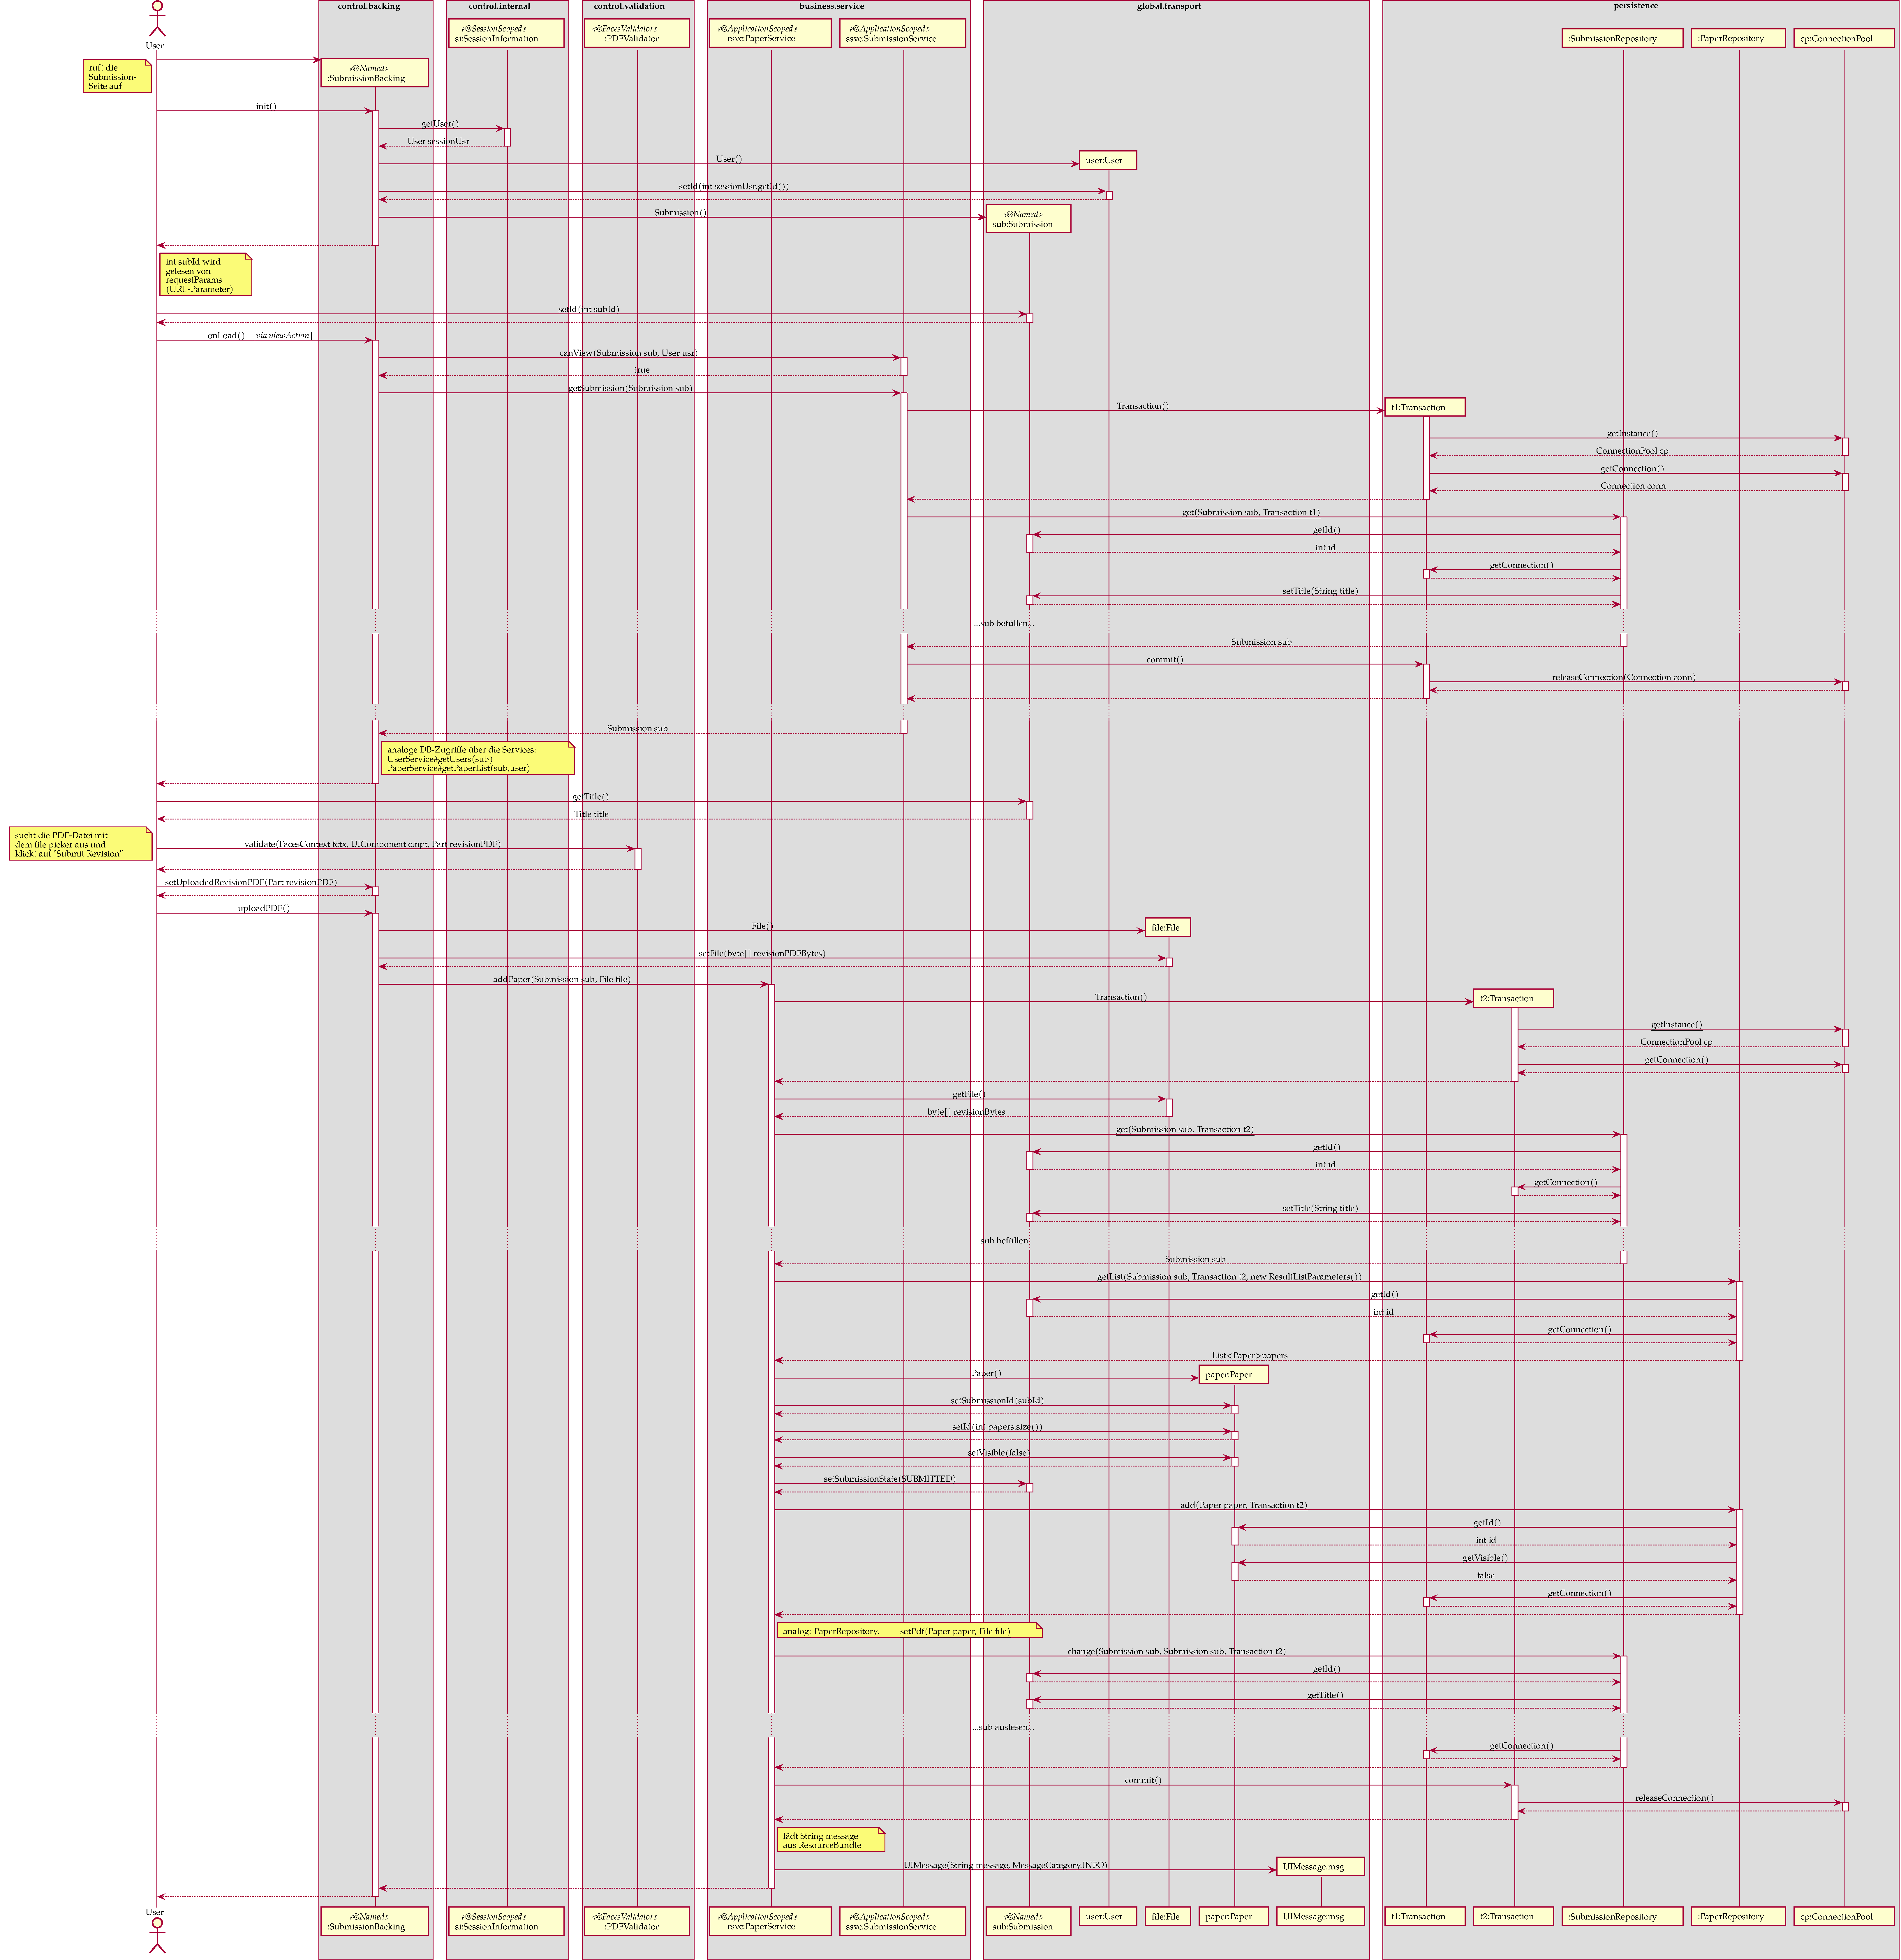
\includegraphics[width=0.9\textwidth]{graphics/upload_revision}
    \caption{Sequenzdiagramm zur Ablehnung einer Einreichung}
    \label{fig:upload-revision-sequence}
\end{figure}

\subsection{Ablehnung einer Einreichung}\label{subsec:sequenz-ablehnung}

Abbildung~\ref{fig:rejection-sequence} zeigt die Interaktionen zwischen den Klassen beim Ablehnen einer Einreichung, die Verbindung zum Datenbankserver schlägt aber fehl und die Einreichung kann nicht verändert werden.
Hier ruft ein Editor die Seite einer Einreichung auf und klickt auf den Button zum Ablehnen.
Beim Datenbankzugriff für die Aktualisierung des Status passiert ein Timeout.
Da dies ein fataler Fehler ist, wird der Nutzer mithilfe des ExceptionHandlers auf eine Fehlerseite weitergeleitet.

\begin{figure}[H]
    \centering
    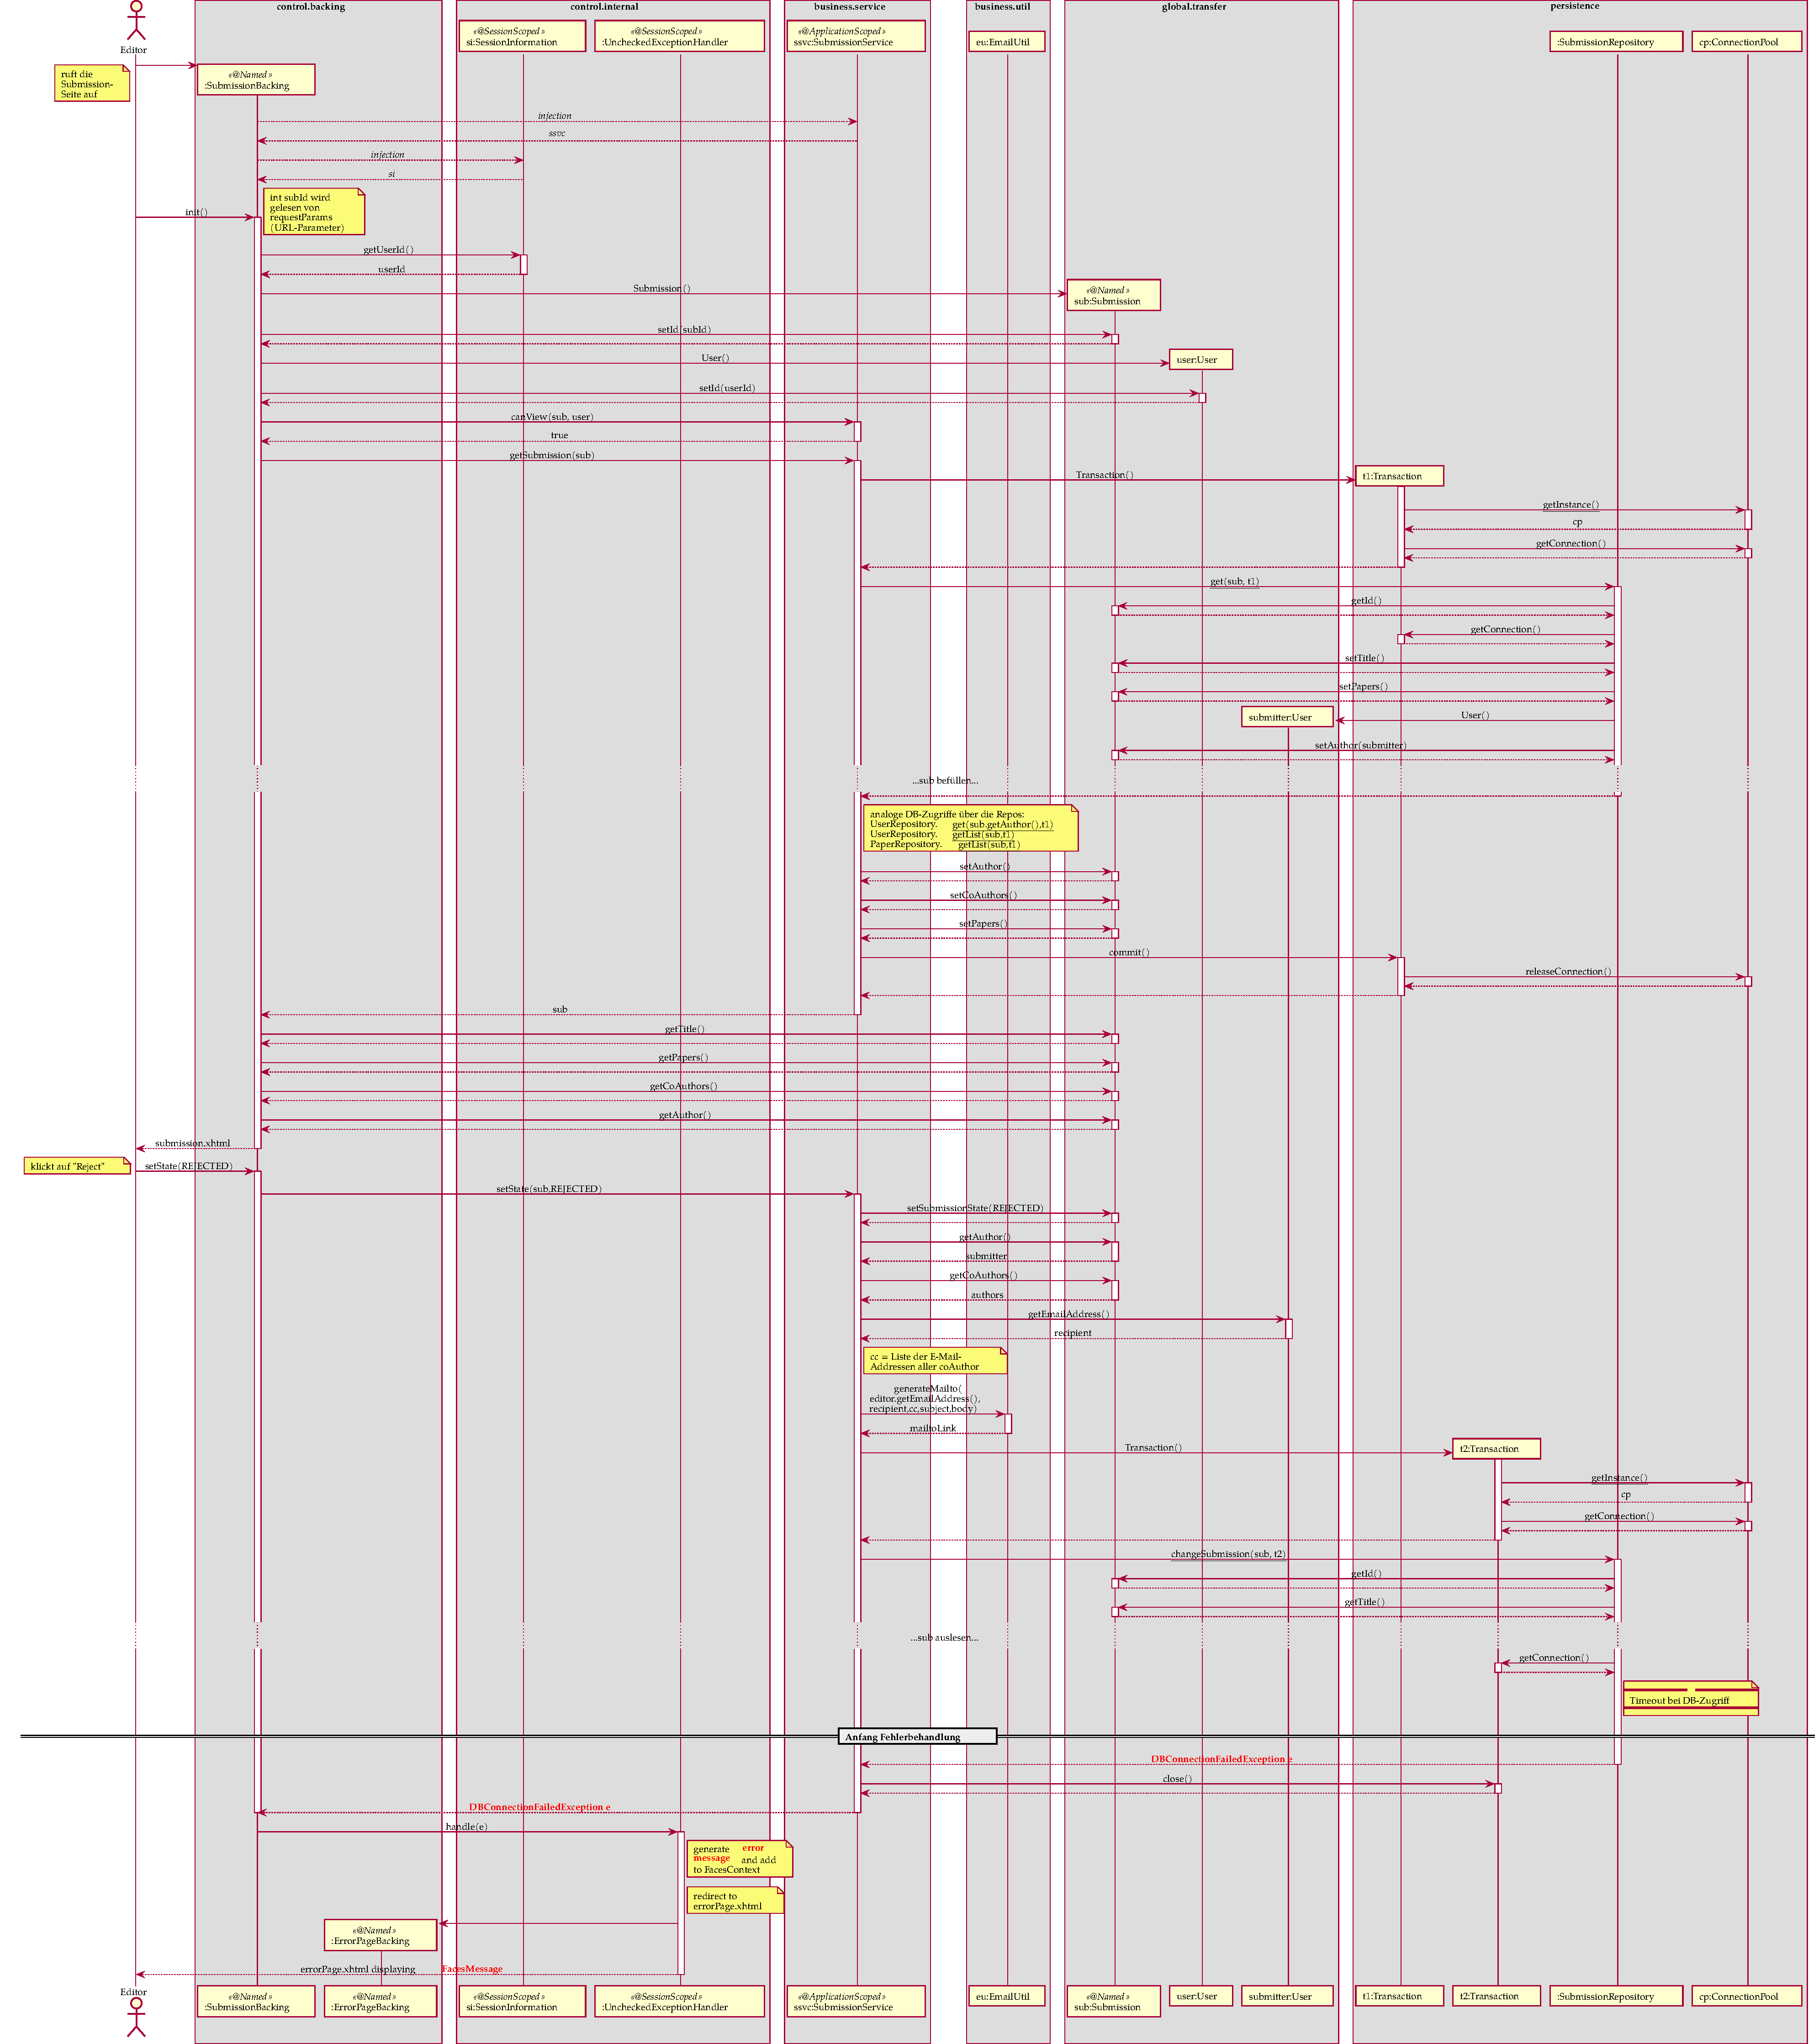
\includegraphics[width=0.9\textwidth]{graphics/reject_submission}
    \caption{Sequenzdiagramm zur Ablehnung einer Einreichung}
    \label{fig:rejection-sequence}
\end{figure}


    \section{Security}\label{sec:security}
    \localauthor{Thomas Kirz}

Im Folgenden wird erklärt, wie verschiedene Sicherheitsangriffe verhindert und Sicherheitsrisiken ausgeschlossen werden.

\subsection{Cross Site Scripting (XSS)}\label{subsec:xss}
Da JSF components für die HTML-Ausgabe verwendet werden, bereinigt JSF alle Nutzereingaben.
Zum Beispiel werden also \code{'<'} und \code{'>'} durch \code{'\&lt;'} und \code{'\&gt;'} ersetzt und Nutzereingaben können keine HTML-Tags in der Ausgabe erstellen.
Dadurch wird XSS bzw.\ HTML-Injection unmöglich.
Auch JavaScript kann so nicht injected werden, da sich JavaScript-Code in einem HTML-Tag (\code{<script>}) befinden müsste.

\subsection{SQL-Injection}\label{subsec:sql-injection}
Für SQL-Code werden \code{PreparedStatements} benutzt, damit die SQL-Statements ohne von Nutzereingaben abhängige Parameter vorkompiliert werden.
Die Parameter werden dann an die Datenbank gesendet und von ihr getrennt vom Code als Daten betrachtet.
Die Ausführung des Statements kann also nicht durch die Nutzereingaben modifiziert werden und eine SQL-Injection wird verhindert

\subsection{Session Hijacking \& Fixation}\label{subsec:session-hijacking}
In der \code{web.xml}-Datei ist ein Timeout für Sessions konfigurierbar.
Dieser wirkt Session Hijacking sowie unerwünschten physischen Zugriffen auf den Browser des Clients entgegen.
JSF setzt für das Session-Cookie standardmäßig das \code{http-only}-Flag, damit kann darauf nicht mit JavaScript zugegriffen werden und Hijacking wird erschwert.

Nach jeder Anmeldung wird die Session verworfen und neu generiert mit
{\small
\begin{lstlisting}
FacesContext.getCurrentInstance().getExternalContext()
    .getRequest().changeSessionId()
\end{lstlisting}
}
Nach einer Authentifizierung bleibt also keine alte Session bestehen und \emph{Session-Fixation}-Attacken werden verhindert.

\subsection{Passwörter}\label{subsec:passwords}
Passwörter werden mit der modernen und sicheren PBKDF2-Funktion gehasht.
Dabei wird für jedes Passwort ein eigener zufällig generierter Salt benutzt, welcher mit dem Hash in der Datenbank gespeichert wird.
Eingegebene Passwörter werden so früh wie möglich gehasht, damit die Klartextpasswörter eine minimale Lebenszeit auf dem Server haben.
Für das Generieren eins Salts und das Hashing bietet die Klasse \code{Hashing} aus \code{de.java.business.util}
Methoden an.
Sie verwendet die robuste \code{javax.crypto}-Bibliothek.

Um das Erraten von Passwörtern durch Brute-Force-Attacken o.ä.\ zu erschweren, müssen Passwörter 8--100 Zeichen lang sein und Groß- und Kleinbuchstaben, Zahlen und Sonderzeichen enthalten.

\subsection{Insecure Direct Object Reference}\label{subsec:idor}
Beim Aufruf von Submission- und Profilseiten werden URL-Parameter benutzt, um die jeweilige Einreichung bzw\. Profil zu identifizieren.
Damit nicht die dafür intern in der Datenbank verwendeten IDs an die Öffentlichkeit (oder einen potentiellen Angreifer) gelangen, werden diese IDs vor der Ausgabe gehasht.
Dafür wird die Klasse \code{Hashing} aus \code{de.java.business.util} benutzt.
Dafür wird ein Hash benutzt, der beim ersten Systemstart generiert und in der Konfigurationsdatei gespeichert wird.
Damit kann von einem Hash nicht auf eine andere ID bzw.\ dessen Hash geschlossen werden.

Unsere Zugangskontrolle \todo{link} sorgt dafür, dass auch bei Erfahren einer ID auf keine Ressourcen illegal zugegriffen werden könnte.

\subsection{Information Leakage}\label{subsec:information-leakage}
Alle Informationen über das System, die nach außen gelangen, können Angreifern helfen.
Dazu gehören Details über die technische Umgebung und verwendete Software des Systems, interne Fehlermeldungen und Implementierungsdetails.
Folgende Maßnahmen werden ergriffen, um Leakage solcher Informationen zu verhindern.
Fehlermeldungen zeigen im Produktionsmodus keine Stacktraces an, sondern eigene Fehlermeldungen, die nur Informationen enthalten, die für den Endnutzer relevant sind.
Wir verwenden eigene Fehlerseiten bei Exceptions und ersetzen die 404-Seite von JSF durch unsere eigene wie folgt in der web.xml-Datei:
    {\small
\begin{lstlisting}
<error-page>
    <error-code>404</error-code>
    <location>/</location>
</error-page>
\end{lstlisting}\todo{location}
}
Dadurch ist nicht ersichtlich, dass wir JSF/Mojarra verwenden.
Das wird auch durch die Verwendung von .xhtml-Dateiendungen für unsere Facelets und Ersetzen des Bezeichners \code{JSESSONID} für Session-Cookies und URL-Rewriting in der web.xml-Datei verborgen:
    {\small
\begin{lstlisting}
<session-config>
    <cookie-config>
        <name>sesssionid</name>
    </cookie-config>
</session-config>
\end{lstlisting}
}

\end{document}
